\chapter{End of chapter exercise solutions}
\label{eoceSolutions}



%_______________
\eocesolch{Introduction to data}



%_______________
%\begin{multicols}{2}

%% 1.1 CASE STUDY: PREVENTING PEANUT ALLERGIES
	
% 1 ODD (OI 1.1)

\eocesol{(a)~Treatment: $10/43 = 0.23 \rightarrow 23\%$. \\
	(b)~Control: $2/46 = 0.04 \rightarrow 4\%$. 
	(c)~A higher percentage of patients in the treatment group were pain 
	free 24 hours after receiving acupuncture. 
	(d)~It is possible that the observed difference between the two group 
	percentages is due to chance.}
	
% 2 EVEN (OI 1.2)

%% 1.2 DATA BASICS

% 3 ODD (OI4, 1.3)

\eocesol{(a)~``Is there an association between air pollution exposure and preterm births?"
	(b)~143,196 births in Southern California between 1989 and 1993.
	(c)~Measurements of carbon monoxide, nitrogen dioxide, ozone, and particulate 
	matter less than 10$\mu g/m^3$ (PM$_{10}$) collected at air-quality-monitoring 
	stations as well as length of gestation.
	Continuous numerical variables. }

% 4 EVEN (OI4, 1.4)

% 5 ODD (OI4, 1.5)

\eocesol{(a)~``Does explicitly telling children not to cheat affect their likelihood to 
	cheat?".
	(b)~160 children between the ages of 5 and 15.
	(c)~Four variables: (1) age (numerical, continuous), (2) sex (categorical), 
	(3) whether they were an only child or not (categorical), (4) whether they 
	cheated or not (categorical).}

% 6 oi_biostat hummingbirds, pset 5

% 7 oi_biostat, from blue_eggs_food

\eocesol{(a)~Control: the group of 16 female birds that received no treatment. Treatment: the group of 16 female birds that were given supplementary diets. \\
	(b)~"Does egg coloration indicate the health of female collared flycatchers?" \\
	(c)~Darkness of blue color in female birds' eggs. Continuous numerical variable.}


% 8 EVEN (OI4, 1.10)

% 9 oi_biostat

\eocesol{(a)~Each row represents a participant. \\
	(b)~The response variable is colon cancer stage. The explanatory variables are the abundance levels of the five bacterial species. \\
	(c)~Colon cancer stage: ordinal categorical variable. Abundance levels of bacterial species: continuous numerical variable.  }

%% 1.3 DATA COLLECTION PRINCIPLES
	
% 10 (OI4, 1.14)

% 11 ODD (OI4, 1.13)	
	
\eocesol{(a)~The population of interest consists of babies born in Southern California. The sample consists of the 143,196 babies born between 1989 and 1993 in Southern California. \\
	(b)~Assuming that the sample is representative of the population of interest, the results of the study can be generalized to the population. The findings cannot be used to establish causal relationships because the study was an observational study, not an experiment.}

	
% 12 oi_biostat
	
% 13 ODD (OI4, 1.15)

\eocesol{(a)~The population of interest consists of asthma patients who rely on medication for asthma treatment. The sample consists of the 600 asthma patients ages 18-69 who participated in the study. \\
	(b)~The sample may not be representative of the population because study participants were recruited, an example of a convenience sample. Thus, the results of the study may not be generalizable to the population. The findings can be used to establish causal relationships because the study is an experiment conducted with control, randomization, and a reasonably large sample size.}


\textD{\newpage}

% 14 EVEN (OI4, 1.30) edited

% 15 oi_biostat, adapted from chicks_antioxidants

\eocesol{(a)~Experiment. \\
	(b)~The experimental group consists of the chicks that received vitamin supplements. The control group consists of the chicks that did not receive vitamin supplements. \\
	(c)~Randomization ensures that there are not systematic differences between the control and treatment groups. Even if chicks may vary in ways that affect body mass and corticosterone levels, random allocation essentially evens out such differences, on average, between the two groups. This is essential for a causal interpretation of the results to be valid.}

% 16 EVEN (OI4, 1.34) edited

% 17 ODD (OI4, 1.21) 

\eocesol{(a)~Observational study. \\
	(b)~Answers may vary. One possible confounding variable is the wealth of a country. A wealthy country's citizens tend to have a higher life expectancy due to a higher quality of life, and the country tends to have a higher percentage of internet users because there is enough money for the required infrastructure and citizens can afford computers. Wealth of a country is associated with both estimated life expectancy and percentage of internet users. Omitting the confounder from the analysis distorts the relationship between the two variables, such that there may seem to be a direct relationship when there is not.}

% 18 EVEN (OI4, 1.22)

% 19 ODD (OI4, 1.23) context edited

\eocesol{(a)~Simple random sampling is reasonable if 500 students is a large enough sample size relative to the total student population of the university. \\
	(b)~Since student habits may vary by field of study, stratifying by field of study would be a reasonable decision. \\
	(c)~Students in the same class year may have more similar habits. Since clusters should be diverse with respect to the outcome of interest, this would not be a good approach.}

% 20 EVEN (OI4, 1.38)

% 21 ODD (OI4, 1.39)

\eocesol{(a)~Non-responders may have a different response to this question, e.g. 
	parents who returned the surveys likely don't have difficulty spending time 
	with their children. \\
	(b)~It is unlikely that the women who were reached at the same address 3 years 
	later are a random sample. These missing responders are probably renters 
	(as opposed to homeowners) which means that they might be in a lower socio-economic class than the respondents. \\
	(c)~This is an observational study, not an experiment, so it is not advisable to draw conclusions about causal relationships. The relationship may be in the other direction; i.e., that these people go running precisely because they do not have joint problems. Additionally, the data are not even sufficient to provide evidence of an association between running and joint problems because data have only been collected from individuals who go running regularly. Instead, a sample of individuals should be collected that includes both people who do and do not regularly go running; the number of individuals in each group with joint problems can then be compared for evidence of an association.}


% 22 EVEN (OI4, 1.28)

% 23 oi_biostat

\eocesol{The lead author's statements are not accurate because he or she drew conclusions about causation (that increased alcohol sales taxes lower rates of sexually transmitted infections) from an observational study. In addition, although the study observed that there was a decline in gonorrhea rate, the lead author generalized the observation to all sexually transmitted infections.}

% 24 EVEN (OI4, 1.40)

% 25 ODD (OI4, 1.41)

\eocesol{(a)~Randomized controlled experiment.
	(b)~Explanatory: treatment group (categorical, with 3 levels). Response variable: 
	Psychological well-being.
	(c)~No, because the participants were volunteers.
	(d)~Yes, because it was an experiment.
	(e)~The statement should say ``evidence'' instead of ``proof''.}


\textD{\newpage}

%% 1.4 NUMERICAL DATA

% 26 EVEN (OI4, 2.8)

% 27 ODD (OI4, 2.7)

\eocesol{(a)~The two distributions have the same median since they have the same middle number when ordered from least to greatest. Distribution 2 has a higher IQR because its first and third quartiles are farther apart than in Distribution~2. \\
	(b)~Distribution 2 has a higher median since it has a higher middle number when ordered from least to greatest. Distribution 2 has a higher IQR because its first and third quartiles are farther apart than in Distribution~1. \\
	(c)~Distribution 2 has a higher median since all values in this distribution are higher than in Distribution 1. The two distributions have the same IQR since the distance between the first and third quartiles in each distribution is the same. \\
	(d)~Distribution 2 has a higher median since most values in this distribution are higher than those in Distribution 1. Distribution 2 has a higher IQR because its first and third quartiles are farther apart than those of Distribution 1.}


% 28 EVEN (OI4, 2.10)

% 29 ODD (OI4, 2.11)

\eocesol{(a)~The distribution is bimodal, with peaks between 15-20 and 25-30. Values range from 0 to 65.  \\
	(b)~The median AQI is about 30. \\
	(c)~I would expect the mean to be higher than the median, since there is some right skewing.}


% 30 oi_biostat, nursing home data, Pset 1, Q1


% 31 ODD (OI4, 2.17)

\eocesol{(a)~The median is a much better measure of the typical amount earned by these 42 
	people. The mean is much higher than the income of 40 of the 42 people. This is 
	because the mean is an arithmetic average and gets affected by the two extreme observations. The median does not get effected as much since it is robust to 
	outliers.
	(b)~The IQR  is a much better measure of variability in the amounts earned by nearly 
	all of the 42 people. The standard deviation gets affected greatly by the two high 
	salaries, but the IQR is robust to these extreme observations.}

% 32 EVEN (OI4, 2.18)

%% 1.5 CATEGORICAL DATA

% 33 oi_biostat

\eocesol{(a)~These data are categorical. They can be summarized numerically in either a frequency table or relative frequency table, and summarized graphically in a bar plot of either counts or proportions. \\
	(b)~The results of these studies cannot be generalized to the larger population. Individuals taking the survey represent a specific subset of the population that are conscious about dental health, since they are at the dentist's office for an appointment. Additionally, there may be response bias; even though the surveys are anonymous, it is likely that respondents will feel some pressure to give a "correct" answer in such a setting, and claim to floss more often than they actually do.}

% 34 EVEN (OI4, 2.22)



%% 1.6 RELATIONSHIPS BETWEEN TWO VARIABLES

% 35 ODD (OI4, 2.1) edited

\eocesol{(a)~Yes, there seems to be a positive association between lifespan and length of gestation. Generally, as gestation increases, so does life span. \\
	(b)~Positive association. Reversal of the plot axes does not change the nature of an association.}

% 36 EVEN (OI4, 2.2)

% 37 oi_biostat

\eocesol{(a)~75\% of the countries have an adolescent fertility rate less than or equal to 75.73 births per 1,000 adolescents. \\
	(b)~It is likely that the observations are missing due to the Iraq War and general instability in the region during this time period. It is unlikely that the five-number summary would have been affected very much, even if the values were extreme; the median and IQR are robust estimates, and the dataset is relatively large, with data from 188 other countries. \\
	(c)~The median and IQR decreases each year, with Q1 and Q3 also decreasing.}

% 38 oi_biostat, citation: stenosis data

% 39 oi_biostat, cite anger_chd paper

\eocesol{(a)~4,371/8,474 = 0.56 $\rightarrow$ 56\% \\
	(b)~110/190 = 0.58 $\rightarrow$ 58\% \\
	(c)~27/633 = 0.04 $\rightarrow$ 4\% \\
	(d)~53/3,110 = 0.02 $\rightarrow$ 2\% \\
	(e)~Relative risk: $\frac{27/633}{53/3,110} = 2.50$. Yes, since the relative risk is greater than 1. A relative risk of 2.50 indicates that individuals with high trait anger are 2.5 times more likely to experience a CHD event than individuals with low trait anger. \\
	(f)~Side-by-side boxplots, since blood cholesterol level is a numerical variable and anger group is categorical.}



\textD{\newpage}




%_______________
\eocesolch{Probability}

%% 2.1 DEFINING PROBABILITY

% 1 ODD (OI4, 3.1) edited

\eocesol{(a)~False. These are independent trials. \\
	(b)~False. There are red face cards. \\
	(c)~True. A card cannot be both a face card and an ace.}

% 2 EVEN (OI4, 3.6)


% 3 oi_biostat

\eocesol{(a)~$\frac{1}{4}$. \\
	Solution 1: A colorblind male has genotype $X^{-}Y$. He must have inherited $X^{-}$ from his mother (probability of $\frac{1}{2}$) and $Y$ from his father (probability of $\frac{1}{2}$). Since these are two independent events, the probability of both occuring is $(\frac{1}{2}) (\frac{1}{2}) = \frac{1}{4}$. \\
	Solution 2: Determine the possibilities using a Punnett square. There are 4 equally likely possibilities, one of which is a colorblind male. Thus, the probability is $\frac{1}{4}$. 
	
	\begin{center}
		\begin{tabular}{ |c|c|c| } 
			\hline
			& $X^{+}$ & $Y$ \\ 
			\hline
			$X^{+}$ & $X^{+}X^{+}$ & $X^{+}Y$ \\ 
			\hline
			$X^{-}$ & $X^{+}X^{-}$ & $X^{-}Y$ \\ 
			\hline
		\end{tabular}
	\end{center}
	(b)~True. An offspring of this couple cannot be both female and colorblind.}

% 4 oi_biostat


% 5 ODD (OI4, 3.11) edited

\eocesol{(a)~0.25. Let $H$ represent the event of being a high school graduate and $F$ represent the event of being a woman. $P(H) = P(H \textrm{ and } W) + P(H \textrm{ and } W^C) = P(H|W)P(W) + P(H|W^C)P(W^C) = (0.20)(0.50) + (0.30)(0.50) = 0.25$. \\
	(b)~0.91.$(A^C) = P(A^C \textrm{ and } W) + P(A^C \textrm{ and } W^C) = (1-0.09) + (1-0.09) = 0.91$. \\
	(c)~0.25. Let $X$ represent the event of having at least a Bachelor's degree, where $B$ represents the event of attaining at most a Bachelor's degree and $G$ the event of attaining at most a graduate or professional degree.  $P(X|W^C) = P(B|W^C) + P(G|W^C) = 0.16 + 0.09 = 0.25$. \\
	(d)~0.26. $P(X|W) = P(B|W) + P(G|W) = 0.17 + 0.09 = 0.26$. \\
	(e)~0.065. Let $X_W$ be the event that a woman has at least a Bachelor's degree, and $X_M$ be the event that a man has at least a Bachelor's degree. Assuming that the education levels of the husband and wife are independent, $P(X_W \textrm{ and } X_M) = P(X_W) \times P(X_M) = (0.25)(0.26) = 0.065$. This assumption is probably not reasonable, because people tend to marry someone with a comparable level of education.
}

% 6 EVEN (OI4, 3.8)


% 7 oi_biostat, from urgent_care_visits

\eocesol{(a)~Let $C$ represent the event that one urgent care center sees 300-449 patients in a week. Assuming that the number of patient visits are independent between urgent care centers in a given county for a given week, the probability that three random urgent care centers see 300-449 patients in a week is $[P(C)]^3 = (0.288)^3 = 0.024$. This assumption is not reasonable because a county is a small area with relatively few urgent care centers; if one urgent care center takes in more patients than usual during a given week, so might other urgent care centers in the same county (e.g., this could occur during flu season). \\
	(b)~$2.32 \times 10^{-7}$. Let $D$ represent the event that one urgent care center sees 450 or more patients in a week. Assuming independence, the probability that 10 urgent care centers throughout a state all see 450 or more patients in a week is $[P(D)]^{10} = (0.217)^{10} = 2.32 \times 10^{-7}$. This assumption is reasonable because a state is a large area that contains many urgent care centers; the number of patients one urgent care center takes in is likely independent of the number of patients another urgent care center in the state takes in. \\
	(c)~No, it is not possible, because it is not reasonable to assume that the patient visits for a given week are independent of those for the following week.}


% 8 EVEN (OI4, 3.12) edited


% 9 ODD (OI4, 3.9)

\eocesol{(a)~If the class is not graded on a curve, they are independent. If graded on a 
	curve, then neither independent nor disjoint -- unless the instructor will only give 
	one A, which is a situation we will ignore in parts~(b) and~(c).
	(b)~They are probably not independent: if you study together, your study habits 
	would be related, which suggests your course performances are also related.
	(c)~No. See the answer to part~(a) when the course is not graded on a curve. More 
	generally: if two things are unrelated (independent), then one occurring does not 
	preclude the other from occurring.}


% 10 EVEN (OI3, 2.18) edited


\textD{\newpage}

%% 2.1 CONDITIONAL PROBABILITY


% 11 ODD (OI4, 3.15)

\eocesol{(a)~$0.60 + 0.20 - 0.18 = 0.62$ \\
	(b)~$0.18/0.20 = 0.90$ \\
	(c)~$0.11/0.33 = 0.33$ \\
	(d)~No, because the answers to parts (c) and (d) are not equal. If global warming belief were independent of political party, then among liberal Democrats and conservative Republicans, there would be equal proportions of people who believe the earth is warming. \\
	(e)~$0.06/0.34 = 0.18$ }

% 12 oi_biostat

% 13 oi_biostat, 2014 brfss data

\eocesol{(a)~$375,264/436,968 = 0.859$ \\
	(b)~$229,246/255,980 = 0.896$ \\
	(c)~0.896. This is equivalent to (b). \\
	(d)~$146,018/180,988 = 0.807$ \\
	(e)~$4,719/7,394 = 0.638$ \\
	(f)~No, because the answers to (c) and (d) are not equal. If gender and seat belt usage were independent, then among males and females, there would be the same proportion of people who always wear seat belts.}

% 14 EVEN (OI4, 3.16)

% 15 ODD (OI3, 2.23), edited

\eocesol{The PPV is 0.8248. The NPV is 0.9728. \\ $P(D|T^{+}) = 
	\frac{P(T^{+}|D)P(D)}{P(T^{+}|D)P(D) + P(T^{+}|D^C)P(D^C)} =  \frac{(0.997)(0.0259)}{(0.997)(0.0259) + (1-0.926)(1-0.259)} = 0.8248$. \\
	\\ $P(D^C|T^{-}) = 
	\frac{P(T^{-}|D^C)P(D^C)}{P(T^{-}|D^C)P(D^C) + P(T^{-}|D)P(D)} =  \frac{(0.926)(1-0.259)}{(0.926)(1-0.259) + (1-0.997)(0.259)} = 0.9728$. \\
	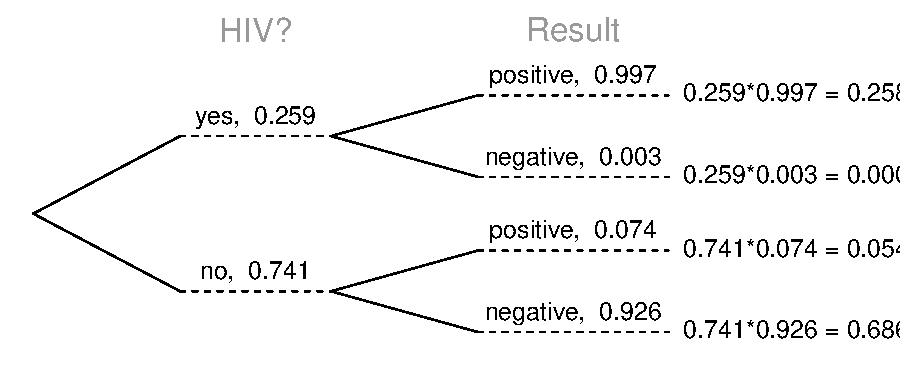
\includegraphics[width=60mm]{ch_probability_oi_biostat/figures/eoce/tree_hiv_swaziland/tree_hiv_swaziland.pdf}}


% 16 EVEN (OI4, 3.18)

% 17 ODD (OI4, 3.21)

\eocesol{0.0714. Even when a patient tests positive for lupus, there is only a 7.14\% 
	chance that he actually has lupus. House may be right.
	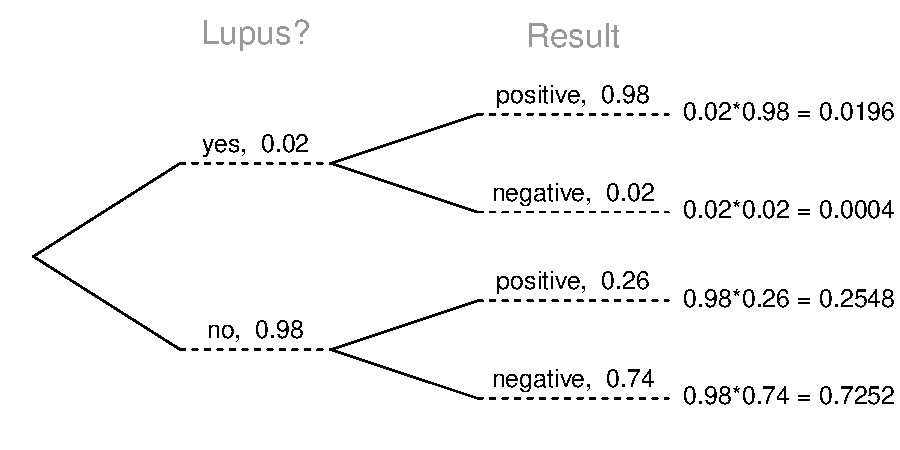
\includegraphics[width=60mm]{ch_probability_oi_biostat/figures/eoce/tree_lupus/tree_lupus.pdf}}


% 18 EVEN (OI4, 3.20) edited

% 19 oi_biostat

\eocesol{(a)~Let $E$ represent the event of agreeing with the idea of evolution and $D$ be the event of being a Democrat. From the problem statement, $P(E|D) = 0.67$. $P(E^C|D) = 1 - P(E|D) = 1 - 0.67 = 0.33$. \\
	(b)~Let $I$ represent the event of being an independent. $P(E|I) = 0.65$, as stated in the problem. \\
	(c)~Let $R$ represent the event of being a Republican. $P(E|R) = 1 - P(E^C|R) = 1 - 0.48 = 0.52$. \\
	(d)~0.35. $P(R|E) = \frac{P(E \textrm{ and }R)}{P(E)} = \frac{P(R)P(E|R)}{P(E)} = \frac{(0.40)(0.52)}{0.60} = 0.35$.}

% 20 oi_biostat, from 2016 final exam

% 21 oi_biostat

\eocesol{Mumps is the most likely disease state, since $P(B_3|A) = 0.563$, $P(B_1|A) = 0.023$, and $P(B_2|A) = .415$. $P(B_i|A) = \frac{P(A|B_i)P(B_i)}{P(A)}$. $P(A) = P(A \textrm{ and } B_1) + P(A \textrm{ and } B_2) + P(A \textrm{ and } B_3) = P(A|B_1)P(B_1) + P(A|B_2)P(B_2) + P(A|B_3)P(B_3)$. \\} 


% 22 EVEN (OI3, 2.26)

% 23 oi_biostat

\eocesol{(a)~Let $A$ be the event of knowing the answer and $B$ be the event of answering it correctly. Assume that if a participant knows the correct answer, they answer correctly with probability 1: $P(B|A) = 1$. If they guess randomly, they have 1 out of $m$ chances to answer correctly, thus $P(B|A^C) = 1/m$. $P(A|B)= \frac{1 \cdot p}{(1 \cdot p) +(\frac{1}{m} \cdot (1-p))} =  \frac{p}{p + \frac{1-p}{m}}$.  \\
	(b)~0.524. Let $A$ be the event of having an IQ over 150 and $B$ be the event of receiving a score indicating an IQ over 150. From the problem statement, $P(B|A) = 1$ and $P(B|A^C) = 0.001$. $P(A^C|B) = \frac{0.001 \cdot (1- \frac{1}{1,100})}{(1 \cdot (\frac{1}{1,100})) + (0.001 \cdot (1- \frac{1}{1,100}))} = 0.524$. }


\textD{\newpage}

% 24 oi_biostat

% 25 oi_biostat

\eocesol{(a)~In descending order on the table, the PPV for each age group is 0.003, 0.064, 0.175, 0.270; the NPV for each age group is 0.999, 0.983, 0.948, 0.914.\\
	(b)~As prevalence of prostate cancer increases by age group, PPV also increases. However, with rising prevalence, NPV decreases.\\
	(c)~The probability that a man has prostate cancer, given a positive test, necessarily increases as the overall probability of having prostate cancer increases. If more men have the disease, the chance of a positive test result being a true positive increases (and the chances of the result being a false positive decreases). The decreasing NPV values follow similar logic: if more men have the disease, the chance of a negative test being a true negative decreases (and the chances of the result being a false negative increases).  \\
	(d)~Lowering the cutoff for a positive test would result in more men testing positive, since men with PSA values 2.5 ng/ml to 4.1 ng/ml were not previously classified as testing positive. Since the sensitivity of a test is the proportion who test positive among those who have disease, and the number with disease does not change, the proportion will increase, except in the rare and unlikely situation where the additional positive tests are among only men without the disease.}


%% 2.3 EXTENDED EXAMPLE

% 26 oi_biostat

% 27 oi_biostat

\eocesol{(a)~Frequency of $X^+X^+$: 0.863. Frequency of $X^+X^-$: 0.132. Frequency of $X^-X^-$: 0.005. Frequency of $X^-Y$: 0.07. Frequency of $X^+Y$: 0.93. From frequency of $X^-X^-$, frequency of $X^-$ allele is $\sqrt{0.005} = 0.071$; thus, frequency of $X^+$ allele is $1 - 0.071 = 0.929$. Frequency of $X^+Y$ is $1 - 0.093 = 0.07$. \\
	(b)~0.033. Let $A$ be the event that two parents are not colorblind, and $B$ represent the event of having a colorblind child. On the tree, $\times$ represents a mating between two genotypes. $P(B|A) = [P(X^{+}X^{+} \times X^{+}Y| A) \cdot P(B |X^{+}X^{+} \times X^{+}Y)] + [P(X^{+}X^{-} \times X^{+}Y| A) \cdot P(B |X^{+}X^{-} \times X^{+}Y)] = (0.867)(0) + (0.133)(1/4) = 0.033$. \\
	\textit{\Tree [.A [.$X^{+}X^{+}$$\times$$X^{+}Y$ [ B $B^C$ ] ] [.$X^{+}X^{-}$$\times$$X^{+}Y$ [ B $B^C$ ] ] ]} \\
}

% 28 oi_biostat, 2020 final exam

% 29 oi_biostat, 2020 midterm exam

\eocesol{(a)~Calculate $P(M \cap B)$, the probability a dog has a facial mask and a black coat. Note that the event $M$ consists of having either a unilateral mask or a bilateral mask.
	
	\begin{align*}
	P(M \cap B) =& P(M_1 \cap B) + P(M_2 \cap B) \\
	=& P(M_1|B)P(B) + P(M_2|B)P(B) \\
	=& (0.25)(0.40) + (0.35)(0.40) \\
	=& 0.24
	\end{align*}
	
	The probability an Australian cattle dog has a facial mask and a black coat is 0.31. \\
	(b)~Calculate $P(M_2)$, the prevalence of bilateral masks. The event of having a bilateral mask can be partitioned into either having a bilateral mask and a red coat or having a bilateral mask and a black coat.
	
	\begin{align*}
	P(M_2) =& P(R \cap M_2) + P(B \cap M_2) \\
	=& P(M_2|R)P(R) + P(M_2|B)P(B) \\
	=& (0.10)(0.60) + (0.35)(0.40)\\
	=& 0.20
	\end{align*}
	
	The prevalence of bilateral masks in Australian cattle dogs is 0.20. \\
	(c)~Calculate $P(R|M_2)$, the probability of having a red coat given having a bilateral mask. Apply the definition of conditional probability.
	
	\begin{align*}
	P(R|M_2) =& \dfrac{P(R \cap M_2)}{P(M_2)} \\
	=& \dfrac{P(M_2|R)P(R)}{P(M_2)} \\
	=& \dfrac{(0.10)(0.60)}{0.20} \\
	=& 0.30
	\end{align*}
	
	The probability of being a Red Heeler among Australian cattle dogs with bilateral facial masks is 0.30. \\
	(d)~The following new information has been introduced: 
	
	- $P(D_1|R, M_0) = P(D_1|R, M_1) = 0.15$, $P(D^C|R, M_0) = P(D^C|R, M_1) = 0.60$.
	
	- $P(M_2 \cap D_2 \cap R) = 0.012$, $P(M_2 \cap D_1 \cap R) = 0.045$
	
	- $P(M_2 \cap D_2 \cap B) = 0.012$, $P(M_2 \cap D_1 \cap B) = 0.045$
	
	- $P(D_1| M_0, B) = P(D_1| M_1, B) = 0.05$, $P(D_2 | M_0, B) = P(D_2 | M_1, B) = 0.01$ \\
	i.~Calculate $P(M_2 \cap D^C \cap R)$.
	
	\begin{align*}
	P(M_2 \cap D^C \cap R) =& P(D^C|M_2, R)P(M_2|R)P(R) \\
	=& \textcolor{red}{P(D^C|M_2, R)}(0.10)(0.60) \\
	\end{align*}
	
	To calculate $P(D^C|M_2, R)$, first calculate $P(D_1|M_2, R)$ and $P(D_2|M_2, R)$ from the joint probabilities given in the problem, then apply the complement rule.
	
	\[P(D_1|M_2, R) = \dfrac{P(M_2 \cap D_1 \cap R)}{P(M_2 \cap R)} = \dfrac{0.045}{(0.10)(0.60)} = 0.75\]
	
	\[P(D_2|M_2, R) = \dfrac{P(M_2 \cap D_2 \cap R)}{P(M_2 \cap R)} = \dfrac{0.012}{(0.10)(0.60)} = 0.20\]
	
	Back to the original question...
	
	\begin{align*}
	P(M_2 \cap D^C \cap R) =& P(D^C|M_2, R)P(M_2|R)P(R) \\
	=& \textcolor{red}{P(D^C|M_2, R)}(0.10)(0.60) \\
	=& [1 - (0.75 + 0.20)](0.10)(0.60) \\
	=& (0.05)(0.10)(0.60) \\
	=& 0.003
	\end{align*}
	
	The probability that an Australian cattle dog has a bilateral mask, no hearing deficits, and a red coat is 0.003. \\
	ii.~Calculate $P(D^C|M_2, B)$.
	
	\begin{align*}
	P(D^C|M_2, B) =& 1 - [P(D_1|M_2, B) + P(D_2|M_2, B)] \\
	=& 1 - \left[ \dfrac{P(D_1 \cap M_2 \cap B)}{P(M_2 \cap B)} + \dfrac{P(D_2 \cap M_2 \cap B)}{P(M_2 \cap B)} \right] \\
	=& 1 - \left[ \dfrac{0.045}{P(M_2|B)P(B)} + \dfrac{0.012}{P(M_2|B)P(B)} \right] \\
	=& 1 - \left[ \dfrac{0.045}{(0.35)(0.40)} + \dfrac{0.012}{(0.35)(0.40)} \right] \\
	=& 0.593
	\end{align*}
	
	The proportion of bilaterally masked Blue Heelers without hearing deficits is 0.593. \\
	iii.~Calculate $P(D|R)$ and $P(D|B)$.
	
	\begin{align*}
	P(D|R) =& P(D \cap M_0|R) + P(D \cap M_1|R) + P(D \cap M_2 |R) \\
	=& [1 - P(D^C|R, M_0)](P(M_0|R) + [1 - P(D^C|R, M_1)](P(M_1|R) + [1 - P(D^C|M_2, R)](P(M_2|R) \\
	=& (1 - 0.60)(0.50) + (1 - 0.60)(0.40) + (1 - 0.05)(0.10) \\
	=& 0.455
	\end{align*}
	
	\begin{align*}
	P(D|B) =& P(D \cap M_0|B) + P(D \cap M_1|B) + P(D \cap M_2 |B) \\
	=& [P(D_1|B, M_0) + P(D_2|B, M_0)](P(M_0|B) + [P(D_1|B, M_0)+ P(D_2|B, M_0)](P(M_1|B) \\
	& \quad  + [1 - P(D^C|M_2, B)](P(M_2|B) \\
	=& (0.05 + 0.01)(0.40) + (0.05 + 0.01)(0.25) + (1 - 0.593)(0.35) \\
	=& 0.181
	\end{align*}
	
	The prevalence of deafness among Red Heelers is higher, at 0.455 versus 0.181 in Blue Heelers. \\
	iv.~Calculate $P(B|D^C)$. 
	
	\begin{align*}
	P(B|D^C) =& \dfrac{P(B \cap D^C)}{P(D^C)} \\
	=& \dfrac{P(D^C|B)P(B)}{P(D^C \cap B) + P(D^C \cap R)} \\
	=& \dfrac{[1 - P(D|B)]P(B)}{[1 - P(D|B)]P(B) + [1 - P(D|R)]P(R)} \\
	=& \dfrac{(1 - 0.181)(0.40)}{(1 - 0.181)(0.40) + (1 - 0.455)(0.60)} \\
	=& 0.50
	\end{align*}
	
	The probability that a dog is a Blue Heeler given that it is known to have no hearing deficits is 0.50.
}


%_______________


\textD{\vspace{10mm}}



%_______________
\eocesolch{Distributions of random variables}

%_______________

%% 3.1 RANDOM VARIABLES

% 1 ODD (OI4, 3.29)

\eocesol{(a)~13.
	(b)~No, these 27 students are not a random sample from the university's student 
	population. For example, it might be argued that the proportion of smokers among 
	students who go to the gym at 9 am on a Saturday morning would be lower than the 
	proportion of smokers in the university as a whole.}

% 2 EVEN (OI4, 3.30)

% 3 ODD (OI4, 3.31) edited

\eocesol{(a)~The probability of drawing three hearts equals $(13/52)(12/51)(11/50) = 0.0129$, and the probability of drawing three black cards equals $(26/52)(25/51)(24/50) = 0.1176$; thus, the probability of any other draw is $1 - 0.0129 - 0.1176 = 0.8694$. $E(X) = 0.0129(50) + 0.1176(25) + 0.8694(0) = 3.589.$ $Var(X) = 0.0129(50-3.589)^2 + 0.1176(25-3.589)^2 + 0.8694(0-3.589)^2 = 93.007$. $SD(X) = \sqrt{Var(X)} = 9.644.$ \\ (b)~Let $Y$ represent the net profit/loss, where $Y = X - 5$. $E(Y) = E(X - 5) = E(X) - 5 = -1.412$. Standard deviation does not change from a shift of the distribution; $SD(Y) = SD(X) = 9.644$. \\
	(c)~It is not advantageous to play, since the expected winnings are lower than \$5.}


% 4 EVEN (OI4, 3.34)

% 5 oi_biostat, incubation_capacity

\eocesol{(a)~215 eggs. Let $X$ represent the number of eggs laid by one gull. $E(X) = 0.25(1) + 0.40(2) + 0.30(3) + 0.05(4) = 2.15.$ $E(100X) = 100E(X) = 215.$ \\
	(b)~85.29 eggs. $Var(X) = 0.25(1-2.15)^2 + 0.40(2-2.15)^2 + 0.30(3-2.15)^2 + 0.05(4-2.15)^2 = 0.7275.$ $Var(100X) = 100^2Var(X) = 7275 \rightarrow \sqrt{7275} = 85.29.$ }

% 6 EVEN (OI3, 2.42)

%% 3.2 BINOMIAL DISTRIBUTION

\textD{\newpage}

% 7 ODD (OI4, 4.17)

\eocesol{(a)~Binomial conditions are met: 
	(1)~Independent trials: In a random sample across the US, it is reasonable to assume that whether or not one 18-20 year old has consumed alcohol does not depend on whether or not another one has.
	(2)~Fixed number of trials: $n = 10$.
	(3)~Only two outcomes at each trial: Consumed or did not consume alcohol.
	(4)~Probability of a success is the same for each trial: $p = 0.697$. \\
	(b)~Let $X$ be the number of 18-20 year olds who have consumed alcohol; $X \sim \textrm{Bin}(10, 0.697)$. $P(X=6) = 0.203$. \\
	(c)~Let $Y$ be the number of 18-20 year olds who have not consumed alcohol; $Y \sim \textrm{Bin}(10, 1-0.697)$. $P(Y = 4) = P(X = 6) = 0.203$. \\
	(d)~$X \sim \textrm{Bin}(5, 0.697)$. $P(X \leq 2) =  0.167$. \\
	(e)~$X \sim \textrm{Bin}(5, 0.697)$. $P(X \geq 1) = 1 - P(X = 0) = 0.997$.}

% 8 EVEN (OI4, 4.18)

% 9 ODD (OI4, 4.19)

\eocesol{(a)~$\mu 34.85$, $\sigma = 3.25$
	(b)~$Z = \frac{45 - 34.85}{3.25} = 3.12$. 45 is more than 3 standard 
	deviations away from the mean, we can assume that it is an unusual 
	observation. Therefore yes, we would be surprised.
	(c)~Using the normal approximation, 0.0009. With 0.5 correction, 0.0015.}

% 10 EVEN (OI4, 4.20)

% 11 oi_biostat, abo_blood

\eocesol{(a)~Both O+ and O- individuals can donate blood to a Type O+ patient; $n = 15$, $p = 0.45$. $\mu = np = 6.75$. $\sigma = \sqrt{np(1-p)} = 1.93$. \\
	(b)~Only O- individuals can donate blood to a Type O- patient; $n = 15$, $p = 0.08$. $P(X \geq 3) = 0.113$.}


% 12 EVEN (OI4, 4.24)

% 13 oi_biostat, 2016 midterm question 1c

\eocesol{0.132. Let $X$ be the number of IV drug users who contract Hepatitis C within a month; $X \sim \textrm{Bin}(5, 0.30)$, $P(X = 3) = 0.132$.}

% 14 EVEN (OI4, 4.22)

% 15 oi_biostat, wolbachia_prevalence

\eocesol{(a)~Let $X$ represent the number of infected stocks in the sample; $X \sim \textrm{Bin}(250, 0.30)$. $P(X = 60) = 0.006$. \\
	(b)~$P(X \leq 60) = 0.021$. \\
	(c)~$P(X \geq 80) = 0.735$. \\
	(D)~40\% of 250 is 100. $P(X \leq 100) = 0.997$. Yes, this seems reasonable; it is essentially guaranteed that within a sample of 250, no more than 40\% will be infected.}

% 16 EVEN (OI4, 4.26)

% 17 oi_biostat, from unit 3 lecture (2016), slide 26

\eocesol{(a)~$(200)(0.12) = 24$ cases of hyponatremia are expected during the marathon. \\
	(b)~Let $X$ represent the number of cases of hyponatremia during the marathon. $P(X > 30) = 0.082$.}


% 18 oi_biostat fall 2019 stat 104 in-class exam

%% 3.3 NORMAL DISTRIBUTION

% 19 ODD (OI4, 4.1)

\eocesol{(a)~8.85\%.
	(b)~6.94\%.
	(c)~58.86\%.
	(d)~4.56\%. \\
	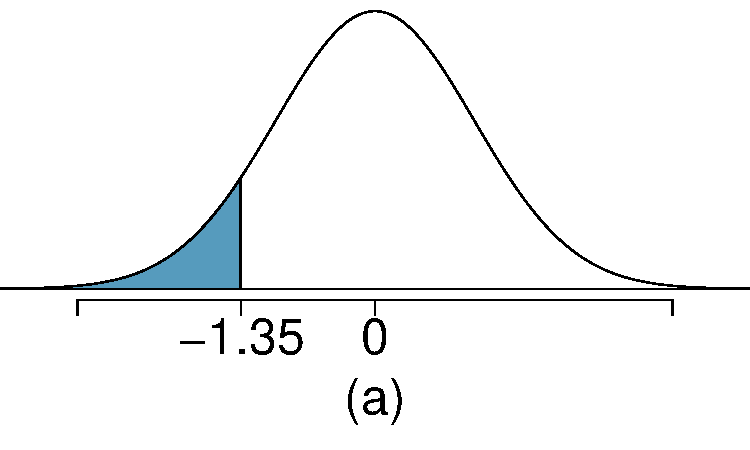
\includegraphics[width=0.23\textwidth]{ch_distributions_oi_biostat/figures/eoce/area_under_curve_1/zltNeg}
	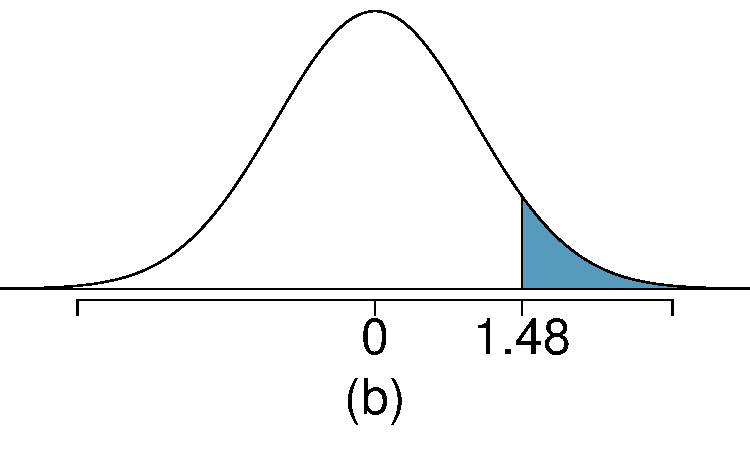
\includegraphics[width=0.23\textwidth]{ch_distributions_oi_biostat/figures/eoce/area_under_curve_1/zgtPos}
	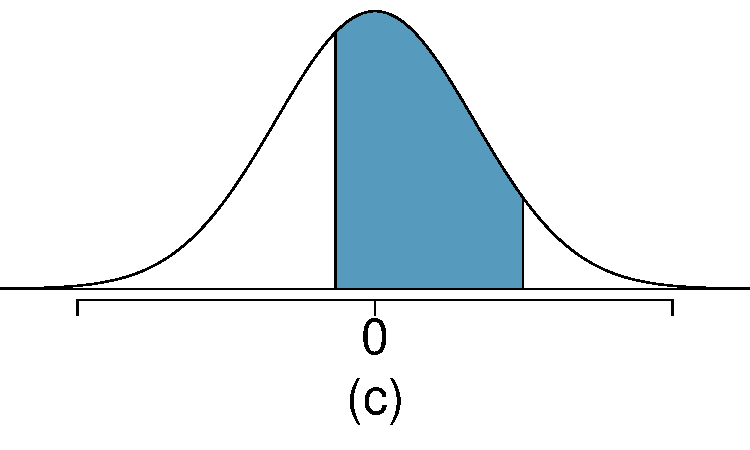
\includegraphics[width=0.23\textwidth]{ch_distributions_oi_biostat/figures/eoce/area_under_curve_1/zBet}
	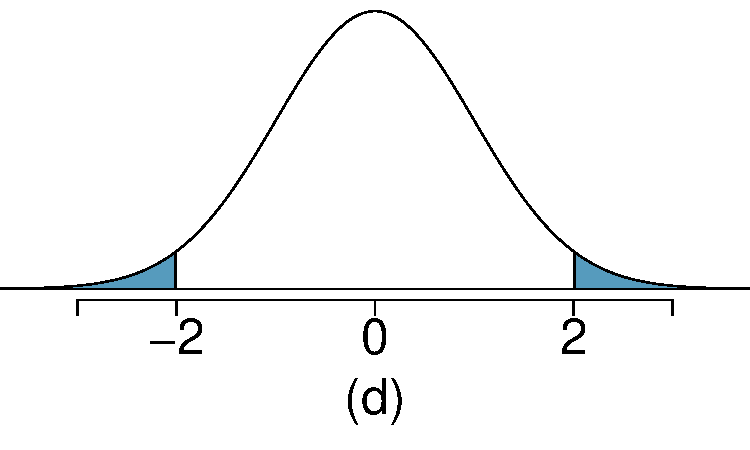
\includegraphics[width=0.23\textwidth]{ch_distributions_oi_biostat/figures/eoce/area_under_curve_1/zgtAbs}}

% 20 EVEN (OI4, 4.2)

% 21 oi_biostat, from pset 3 (2016), problem 7

\eocesol{(a)~0.005. (b)~0.911. (c)~0.954. (d)~1.036. (e)~-0.842}

% 22 EVEN (OI3, 3.4, 3.6) edited

% 23 ODD (OI3, 3.3, 3.5) edited

\eocesol{(a)~Verbal: $N(\mu = 151, \sigma = 7)$, Quant: $N(\mu = 153, \sigma = 7.67)$. $Z_{VR} = 1.29$, $Z_{QR} = 0.52$. She did better on the Verbal Reasoning section since her Z-score on that 
	section was higher.\\
	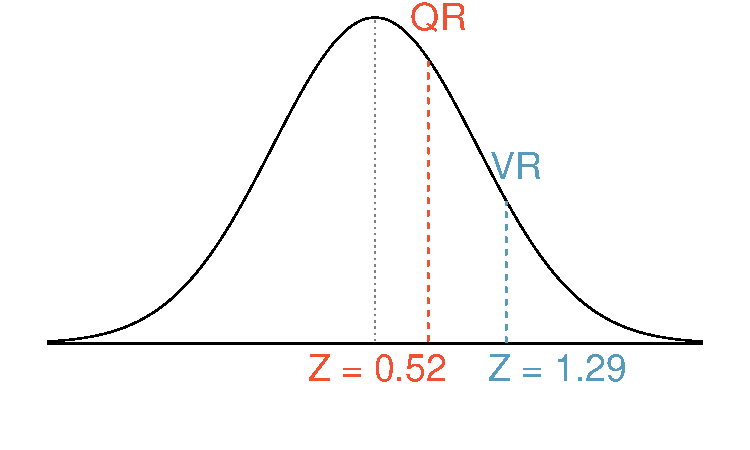
\includegraphics[width=0.3\textwidth]{ch_distributions_oi_biostat/figures/eoce/gre_intro/gre_intro.pdf} \\
	(b)~$Perc_{VR} = 0.9007 \approx 90\%$, $Perc_{QR} = 0.6990 \approx 70\%$. $100\% - 90\% = 10\%$ did better than her on VR, and $100\% - 70\% = 30\%$
	did better than her on QR. \\
	(c)~159.
	(d)~147.}

% 24 oi_biostat, from pset 3 (2016), problem 8

% 25 ODD (OI4, 4.7) edited

\eocesol{(a)~0.115. (b)~The coldest 10\% of days are colder than 70.59\degree F.}

% 26 oi_biostat, clutch_volume

% 27 oi_biostat, 2016 midterm exam, problem 1a

\eocesol{(a)~0.023. (b)~72.66 mg/dL.}

% 28 oi biostat, pset 3 (2016), problem 9

\textD{\newpage}

% 29 oi_biostat, unit 3 lecture slides (2016), slide 11

\eocesol{(a)~82.4\%. (b)~About 38 years of age.}

% 30 EVEN (OI3, 3.14)

% 31 ODD (OI3, 3.27) edited

\eocesol{(a)~$n = 50$, and $p = 0.70$. $\mu = np = 35$. $\sigma = \sqrt{np(1-p)} = 3.24$. \\
	(b)~Both $np$ and $n(1-p)$ are greater than 10. Thus, it is valid to approximate the distribution as $X \sim N(35, 3.24)$, where $X$ is the number of 18-20 year olds who have consumed alcohol. $P(X \geq 45) = 0.001$. }

% 32 EVEN (OI4, 3.28) edited

% 33 ODD (OI3, 3.29)

\eocesol{Let $X$ represent the number of students who accept the offer; $X \sim \textrm{Bin}(2500, 0.70)$. This distribution can be approximated by a $N(1750, 22.91)$. The approximate probability that the school does not have enough dorm room spots equals $P(X \geq 1,786) = 0.06$.}

% 34 EVEN (OI3, 3.16)

% 35 ODD (OI3, 3.17) edited

\eocesol{The data appear to follow a normal distribution, since the points closely follow the line on the normal probability plot. There are some small deviations, but this is to be expected for such a small sample size.}

	
% 36 EVEN (OI3, 3.18) edited

%% 3.4 POISSON DISTRIBUTION

% 37 oi_biostat

\eocesol{(a)~$P(X = 2) = \frac{\exp^{-2}(2^2)}{2!} = 0.271$. (b)~$P(X \leq 2) = P(X = 0) + P(X = 1) + P(X = 2) = 0.677$. (c)~$P(X \geq 3) = 1 - P(X \leq 2) = 0.323$.}

% 38 EVEN (OI4, 4.32) edited

% 39 ODD (OI4, 4.31) edited

\eocesol{(a)~$\mu=\lambda=75$, $\sigma=\sqrt{\lambda} = 8.66$.
	(b)~$Z=-1.73$. Since 60 is within 2 standard deviations of the mean, it would not generally be considered unusual. Note that we often use this rule of thumb even when the normal model does not apply.
	(c)~Using Poisson with $\lambda = 75$: 0.0402.}

% 40 oi_biostat, pset 3 (2020), problem 5

% 41 ODD (OI4, 4.33)

\eocesol{(a)~The expected number of cases of osteosarcoma in NYC in a given year is 11.2.
	(b)~Let $X$ represent the number of osteosarcoma cases diagnosed. The probability that 15 or more cases will be diagnosed in a given year is the quantity $P(X \geq 15) = 1 - P(X < 15) = 1 - P(X \leq 14) = 0.161.$
	(c)~First, calculate $\lambda_B$ given that $n=450,000$ for Brooklyn: 3.6. The probability of observing 10 or more cases in Brooklyn in a given year is the quantity $P(X_B\geq 10)= 1-P(X_B<10)=1-P(X_B\leq 9) = 0.004.$
	(d)~No, he is not correct. The probability calculated in c) deals only with Brooklyn: the probability that there are 10 or more cases in Brooklyn for a single year. It does not say anything about cases in other boroughs. If we assume independence between boroughs, the probability that the official is referring to is:
	
	$P(X = 0 \ \text{in other boroughs}) \times P(X \geq 10 \ \text{in Brooklyn})$.
	
	There is no reason to expect that $P(X = 0 \ \text{in other boroughs})$ should equal 1, so this probability is different from the one in part c).
	(e)~o, this probability is not equal to the probability calculated in part c). Over five years, there are five opportunities for the event of 10 or more cases in Brooklyn in a single year to occur. Let $Y$ represent the event that in a single year, 10 or more cases of osteosarcoma are observed in Brooklyn. If we assume independence between years, then $Y$ follows a binomial distribution with $n = 5$ and $p$ of success as caculated in part c); $P(Y = 1) = 0.020$.
}

% 42 EVEN (OI4, 4.34)

% 43 oi_biostat

\eocesol{(a)~$\lambda$ for a population of 2,000,000 male births is 400. The probability of at most 380 newborn males with hemophilia is $P(X \leq 380$), where $X \sim \textrm{Pois}(400)$: 0.165. \\
	(b)~$P(X \geq 450) = 0.0075$. \\
	(c)~The number of male births is (1/2)(1,500,000) = 750,000. The rate $\lambda$ for one year is 150. Over 5 years, the rate $\lambda$ is 750. The expected number of hemophilia births over 5 years is 750 and the standard deviation is $\sqrt{750} = 27.39$.}

% 44 oi_biostat, 2016 midterm, question 3

%% 3.5 DISTRIBUTIONS RELATED TO BERNOULLI TRIALS

%%geometric distribution

% 45 ODD (OI3, 3.21)

\eocesol{(a)~On average, 2 women would need to be sampled in order to select a married woman ($\mu = 1/p = 2.123$), with standard deviation 1.544 ($\sigma = \sqrt{\frac{(1-p)}{p^2}}$). \\
	(b) $\mu = 3.33$. $\sigma = 2.79$. \\
	(c)~Decreasing the probability increases both the mean and the standard deviation. }

% 46 oi_biostat, abo_blood

% 47 oi_biostat, wolbachia_prevalence

\eocesol{(a)~Let $X$ represent the number of stocks that must be sampled to find an infected stock; $X \sim \textrm{Geom}(0.30)$. $P(X \leq 5) = 0.832$.\\
	(b)~$P(X \leq 6) = 0.882$.\\
	(c)~$P(X \geq 3) = 1 - P(X \leq 2) = 0.49$. }

% 48 EVEN (OI4, 4.12)

\textD{\newpage}

% 49 ODD (OI4, 4.13) edited 

\eocesol{(a)~$0.875^2\times 0.125 = 0.096$.
	(b)~$\mu=8$, $\sigma=7.48$.}

% 50 EVEN (OI4, 4.14)

%% negative binomial

% 51 ODD (OI4, 4.27)

\eocesol{(a)~0.0804.
	(b)~0.0322.
	(c)~0.0193.}

% 52 EVEN (OI4, 4.28) edited

% 53 oi_biostat, cilantro_pref

\eocesol{(a)~0.102, geometric with $p = 1994/14,604 = 0.137$.\\
	(b)~0.854, binomial with $n = 10$, $p = 0.137$.\\
	(c)~0.109, binomial with $n = 10$, $p = 0.137$.\\
	(d)~The mean and standard deviation of a negative binomial random variable with $r = 4$ and $p = 0.137$ are 29.30 and 13.61, respectively.}

% 54 EVEN (OI4, 4.30) edited

%% hypergeometric problems

% 55 oi_biostat

\eocesol{(a)~$\mu = 2.05$; $\sigma^2 = 1.77$. \\
	(b)~Let $X$ represent the number of soapy-taste detectors; $X \sim \textrm{HGeom}(1994, 14604-1994,15)$. $P(X = 4) = 0.09435$.\\
	(c)~$P(X \leq 2) = 0.663$.\\
	(d)~0.09437, from the binomial distribution. With a large sample size, sampling with replacement is highly unlikely to result in any particular individual being sampled again. In this case, the hypergeometric and binomial distributions will produce equal probabilities.}

% 56 oi_biostat, flanders_caries

% 57 oi_biostat

\eocesol{(a)~The marginal distributions for $X$ is obtained by summing across the two rows, and for $Y$ by summing the columns.  The marginal probabilities for $X = 0$ and $X = 1$ are 0.60 and 0.40, and for $Y = -1$ and $Y = 1$ are both 0.50; i.e., $p_X(0) = 0.60$, $p_X(1) = 0.40$, $p_Y(-1) = p_Y(1) = 0.50$
	(b)~The mean and variance of $X$ are calculated using the formulas in Section~\ref{section:expectationRandomVariable} and \ref{section:varianceRandomVariable} and are 
	\begin{align*}
	\mu_X &= (0)(0.60) + (1)(0.40) = 0.40 \\
	\sigma^2_X &= (0 - 0.40)^2 (0.60) + (1 - 0.40)^2(0.40) = 0.24
	\end{align*}
	The standard deviation of $X$ is $\sqrt{0.24} = 0.49$.
	(c)~The two standardized values of $X$ are obtained by subtracting the mean of $X$ from each value and dividing by the standard deviation.  The two standardized values are -0.82 and 1.23.
	(d)~The correlation between $X$ and $Y$ adds the 4 products of the standardized values, weighted by the values in the joint distribution:
	\[\rho_{X,Y} = (-0.82)(-1)(0.20) + (-0.83)(1)(0.40) + (1.23)(-1)(0.30) + (1.23)(1)(0.10) = -.41 \]
	(e)~No.  The correlation between $X$ and $Y$ is not zero.
}


% 58 oi_biostat

% 59 oi_biostat

\eocesol{(a)~Sum over the margins to calculate the marginal distributions.
	\[p_Y(-1) = 0.25 \quad p_Y(0) = 0.20 \quad p_Y(1) = 0.55 \]
	\[p_X(-1) = 0.45 \quad p_X(0) = 0.20 \quad p_X(1) = 0.35 \]
	(b)~The expected value of $X$ is calculated as follows:
	\[E(X) = \sum_i x_i P(X = x_i) = (-1)(0.45) + (0)(0.20) + (1)(0.35) = -0.10 \]
	(c)~The variance of $Y$ is calculated by first calculating $E(Y)$, then using that in the formula for a variance of a random variable.
	\[E(Y) = \sum_i y_i P(Y = y_i) = (-1)(0.25) + (0)(0.20) + (1)(0.55) = 0.30 \]
	\[\text{Var}(Y) = \sum_i (y_i - E(Y))^2 P(Y = y_i) = (-1 - 0.30)^2(0.25) + (0 - 0.30)^2(0.20) + (1 - 0.30)^2(0.55) = 0.71\]
	(d)~$P(X = -1|Y = 0) = 0/0.20 = 0$; $P(X = 0 | Y = 0) = 0.10/0.20 = 0.50$; $P(X = 1|Y = 0) = 0.10/0.20 = 0.5$.}


% 60 oi_biostat

\textD{\newpage}

% 61 oi_biostat

\eocesol{(a)~No.  The new marginal distributions for the costs for the two members of the couple are shown in the following table. The values and the marginal distribution for the partner's cost do not change, so the expected value and standard deviation will not change.  The previous values for the mean and standard deviation were \$980 and \$9.80.
	
	\begin{center}
		\begin{tabular}{c|rr | c}
			&   \multicolumn{2}{c}{\textbf{Partner Costs, $Y$}} & \\
			\hline
			\textbf{Employee costs, $X$} & \textbf{\$968} & \textbf{\$988} &  \textbf{Marg. Dist., $X$} \\ 
			\hline
			\textbf{\$968} & 0.18 & 0.12 & 0.30\\ 
			\textbf{\$1,008} & 0.15 & 0.25 & 0.40 \\ 
			\textbf{\$1,028}  & 0.07 & 0.23 & 0.30\\ 
			\hline
			\textbf{Marg. Dist., $Y$} & 0.40 & 0.60 & 1.00 \\
		\end{tabular}
	\end{center}
	(b)~The expected value and standard deviation of the employee's costs are calculated as in Example~\ref{example:healthCareCosts}, but using the new marginal distribution.  The new values for the mean and standard deviation are \$1,002 and \$23.75.
	(c)~The expected total cost is \$1,002 + \$980 = \$1,982.
	(d)~The calculation correlation depends on the standardized costs for each member of the couple and the joint probabilities. The new standardized values for the employee costs are -1.43, 0.25, and 1.09; the corresponding values for the partner are -1.22 and 0.82.  The correlation is the weighted sum of the 6 products, weighted by the joint probabilities: $\rho_{X, Y} = 0.29$.
	(e)~The new variance for the total cost will be $(23.80)^2 + (9.80)^2 + (2)(23.8)(9.80)(0.29) = 796.00$ The new standard deviation is $\sqrt{796.00} = \$28.21$. 
}


\textD{\vspace{10mm}}



%%%%%%%%%%%%%%%%%%%%%%%%%%%%%%%%%%%%%%%%%%%%%%%%%%%%%%%%%%%%%%%%%%%%%%%%%%%%%%%%%%%%%%%%%%%%%%%%%%%%%%%%%%%%%%

%_______________
\eocesolch{Foundations for inference}



%_______________

%% 4.1 SAMPLING VARIABILITY

% 1 oi_biostat, blue_eggs

\eocesol{(a)~$\overline{x} = 0.6052.$ \\
	(b)~$s = 0.0131$. \\
	(c)~$Z_{0.63} = \frac{0.63 - 0.6052}{0.0131} = 1.893$. No, this level of BGC is within 2 SD of the mean. \\
	(d)~The standard error of the sample mean is given by $\frac{s}{\sqrt{n}} = \frac{0.0131}{\sqrt{70}} = 0.00157$.
}

% 2 EVEN (OI 4.4) edited

% 3 ODD (OI3, 4.5)

\eocesol{(a)~This is the sampling distribution of the sample mean. \\
	(b)~The sampling distribution will be normal and symmetric, centered around the theoretical population mean $\mu$ of the number of eggs laid by this hen species during a breeding period. \\
	(c)~The variability of the distribution is the standard error of the sample mean:  $\frac{s}{\sqrt{n}} = \frac{18.2}{\sqrt{45}} = 2.71$. \\
	(d)~The variability of the new distribution will be greater than the variability of the original distribution. Conceptually, a smaller sample is less informative, which leads to a more uncertain estimate. This can be shown concretely with a calculation: $\frac{18.2}{\sqrt{10}} = 5.76$ is larger than 2.71.
}


%% 4.2 CONFIDENCE INTERVALS

% 4 EVEN (OI3, 4.12)

% 5 ODD (OI3, 4.11) edited

\eocesol{(a)~The mean number of days US residents experienced poor mental health during the past 30 days is contained within the interval (3.40, 4.24) days. \\
	(b)~In this context, 95\% confident implies that 950 out of 1,000 intervals constructed are expected to contain the true mean number of days US residents experienced poor mental health during the past 30 days. \\
	(c)~A 99\% interval will be larger than the 95\% confidence interval. \\
	(d)~The standard error of the estimate would be larger, since 500 individuals is fewer than 1,151 individuals. Reducing sample size increases the standard error.
}

% 6 EVEN (OI3, 4.14) edited

\textD{\newpage}

% 7 ODD (OI3, 4.13) edited

\eocesol{(a)~False. Provided the data distribution is not very strongly skewed ($n = 64$ in 
	this sample, so we can be slightly lenient with the skew), the distribution of the sample mean will 
	be nearly normal, allowing for the normal approximation. \\
	(b)~False. Inference is made on the population parameter, not the point 
	estimate. The point estimate is always in the confidence interval. \\
	(c)~True. \\
	(d)~False. The confidence interval is not about a sample mean. \\
	(e)~False. A wider interval is required to be more confident about capturing the parameter. \\
	(f)~True. The margin of error is half the width of the interval, 
	and the sample mean is the midpoint of the interval. \\
	(g)~False. To halve the margin of 
	error requires sampling $2^2 = 4$ times the number of people in 
	the initial sample.}

% 8 EVEN (OI3, 4.16)

% 9 oi_biostat section 5 spring 2020

\eocesol{(a) i.~False. There is a 5\% chance that any 95\% confidence interval does not contain the true population mean days out of the past 30 days that U.S. adults experienced poor mental health.
	ii.~False. The population parameter $\mu$ is either inside or outside the interval; there is no probability associated with whether the fixed value $\mu$ is in a certain calculated interval. The randomness is associated with the interval (and the method for calculating it), not the parameter $\mu$. Thus, it would not be reasonable to say there is a 95\% chance that the particular interval (3.40, 4.24) contains $\mu$; this interpretation is coherent with the statement in part iii. of this question.
	iii.~True. This is the definition of what it means to be 95\% confident.
	iv.~True. The interval corresponds to a two-sided test, with $H_0: \mu = 4.5$ days and $H_A: \mu \neq 4.5$ days and $\alpha = 1 - 0.95 = 0.05$. Since $\mu_0$ of 4.5 days is outside the interval, the sample provides sufficient evidence to reject the null hypothesis and accept the alternative hypothesis.
	v.~False. We can only be confident that 95\% of the time, the entire interval calculated contains $\mu$. It is not possible to make this statement about $\overline{x}$ or any other point within the interval.
	vi.~False. The confidence interval is a statement about the population parameter $\mu$, the mean days out of the past 30 days that all US adults experienced poor mental health. The sample mean $\overline{x}$ is a known quantity.
	(b)~The 90\% confidence interval will be smaller than the 95\% confidence interval. If we are less confident that an interval contains $\mu$, this implies that the interval is less wide; if we are more confident, the interval is wider. Think about a theoretical "100\%" confidence interval---to be 100\% confident of capturing $\mu$, then the range must be all possible numbers that $\mu$ could be.
	(c)~(3.47, 4.17) \text{ days}
}

% 10 oi_biostat pset 4, spring 2020

%% 4.3 HYPOTHESIS TESTING

% 11 ODD (OI3, 4.17)

\eocesol{(a)~The null hypothesis is that New Yorkers sleep an average of 8 hours of night ($H_0: \mu = 8$ hours). The alternative hypothesis is that New Yorkers sleep less than 8 hours a night on average ($H_A: \mu < 8$ hours). \\
	(b)~The null hypothesis is employees spend on average 15 minutes on non-business activities in a day ($H_0: \mu = 15$ minutes). The alternative hypothesis is that employees spend on average more than 15 minutes on non-business activities in a day ($H_A: \mu > 15$ minutes).
}

% 12 EVEN (OI3, 4.18)

% 13 ODD (OI3, 4.19)

\eocesol{Hypotheses are always made about the population parameter $\mu$, not the sample mean $\overline{x}$. The correct value of $\mu_0$ is 10 hours, as based on the previous evidence; both hypotheses should include $\mu_0$. The correct hypotheses are $H_0: \mu = 10$ hours and $H_A: \mu > 10$ hours. 
} 

% 14 EVEN (OI3, 4.20)

% 15 ODD (OI3, 4.21)

\eocesol{(a)~This claim is not supported by the confidence interval. 3 hours corresponds to a time of 180 minutes; there is evidence that the average waiting time is lower than 3 hours. \\
	(b)~2.2 hours corresponds to 132 minutes, which is within the interval. It is plausible that $\mu$ is 132 minutes, since we are 95\% confident that the interval (128 minutes, 147 minutes) contains the average wait time. \\
	(c)~Yes, the claim would be supported based on a 99\% interval, since the 99\% interval is wider than the 95\% interval.
}

% 16 EVEN (OI3, 4.24)

% 17 ODD (OI3, 4.23)

\eocesol{$H_0: \mu = 130$ grams, $H_A: \mu \neq 130$ grams. Test the hypothesis by calculating the test statistic: $t = \frac{\overline{x} - \mu_0}{s/\sqrt{n}} = \frac{130 - 134}{17/sqrt{35}} = 1.39$. This results in a $p$-value of 0.17. There is insufficient evidence to reject the null hypothesis. There is no evidence that the nutrition label does not provide an accurate measure of calories.
}

% 18 EVEN (OI3, 4.25) edited

\textD{\newpage}

% 19 oi_biostat, pset_04, spring 2016

\eocesol{(a)~The 95\% confidence interval is $3,150 \pm (1.96 \times 250/\sqrt{50}) = (3080.7, 3219.3)$ grams. \\
	(b)~She will conduct a test of the null against the two-sided alternative $H_A: \mu \neq 3250$ grams. Calculate the test statistic: $t = \frac{\overline{x} - \mu_0}{s/\sqrt{n}} = \frac{3150 - 3250}{250/\sqrt{50}} = -2.83$. The $p$-value is 0.007. There is sufficient evidence to reject the null hypothesis and conclude that the mean birthweight of babies from inner-city teaching hospitals is lower than 3,260 grams.
}

% 20 EVEN (OI3, 4.26)

% 21 ODD (OI3, 4.29)

\eocesol{(a)~$H_0$: Anti-depressants do not help symptoms of fibromyalgia. $H_A$: Anti-
	depressants do treat symptoms of fibromyalgia. 
	(b)~Concluding that anti-depressants work for the treatment of fibromyalgia 
	symptoms when they actually do not.
	(c)~Concluding that anti-depressants do not work for the treatment of 
	fibromyalgia symptoms when they actually do.
	(d) If she makes a Type 1 error, she will continue taking medication that does not actually treat her disorder. If she makes a Type 2 error, she will stop taking medication that could treat her disorder.}

% 22 EVEN (OI3, 4.30)

% 23 ODD (OI3, 4.31)

\eocesol{(a)~The standard error is larger under scenario I; standard error is larger for smaller values of $n$. \\
	(b)~The margin of error is larger under scenario I; to be more confidence of capturing the population parameter requires a larger confidence interval. \\
	(c)~The $p$-value from a Z-statistic only depends on the value of the Z-statistic; the value is equal under the scenarios. \\
	(d)~The probability of making a Type II error and falsely rejecting the alternative is higher under scenario I; it is easier to reject the alternative with a high $\alpha$.  
}

% 24 EVEN (OI3, 4.32)



\textD{\vspace{10mm}}


\eocesolch{Inference for numerical data}

% 1 ODD (OI4 7.1)

\eocesol{(a)~$df=6-1=5$, $t_{5}^{\star} = 2.02$ (column with two tails of 0.10, 
	row with $df=5$).
	(b)~$df=21-1=20$, $t_{20}^{\star} = 2.53$ (column with two tails of 0.02, 
	row with $df=20$).
	(c)~$df=28$, $t_{28}^{\star} = 2.05$.
	(d)~$df=11$, $t_{11}^{\star} = 3.11$.}

% 2 ODD (OI4 7.3)

% 3 oi_biostat

\eocesol{On a $z$-distribution, the cutoff value for the upper 5\% of values is 1.96. A $t$-distribution has wider tails than a normal distribution but approaches the shape of a standard normal as degrees of freedom increases. Thus, 1.98 corresponds to the cutoff for a $t$-distribution with 100 degrees of freedom, 2.01 the cutoff for 50 degrees of freedom, and 2.23 the cutoff for 10 degrees of freedom.}

% 4 EVEN (OI4 7.4)

% 5 ODD (OI4 7.5)

\eocesol{The mean is the midpoint: $\bar{x} = 20$. Identify the margin of error: 
	$ME = 1.015$, then use $t^{\star}_{35} = 2.03$ and $SE=s/\sqrt{n}$ in the 
	formula for margin of error to identify $s = 3$.}

% 6 EVEN (OI4 7.6)

% 7 ODD (OI4 7.7)

\eocesol{(a)~$H_0$: $\mu = 8$ (New Yorkers sleep 8 hrs per night on average.) 
	$H_A$: $\mu \neq 8$ (New Yorkers sleep less or more than 8 hrs per
	night on average.)
	(b)~Independence: The sample is random.
	The min/max suggest there are no concerning outliers.
	$T = -1.75$. $df=25-1=24$.
	(c)~ p-value $= 0.093$.
	If in fact the true population mean of the 
	amount New Yorkers sleep per night was 8 hours,
	the probability of getting a 
	random sample of 25 New Yorkers where the average
	amount of sleep is 7.73 hours
	per night or less (or 8.27 hours or more) is 0.093.
	(d)~Since p-value $>$ 0.05, do not reject $H_0$.
	The data do not provide strong evidence that
	New Yorkers sleep more or less than 8 hours per night
	on average.
	(e)~No, since the p-value is smaller than $1 - 0.90 = 0.10$.}

% 8 EVEN (OI4 7.8)

% 9 ODD (OI4 7.9)

\eocesol{$T$ is either -2.09 or 2.09.
	Then $\bar{x}$ is one of the following:
	\begin{align*}
	-2.09 &= \frac{\bar{x} - 60}{\frac{8}{\sqrt{20}}} \ \rightarrow \ \bar{x} = 56.26 \\
	2.09 &= \frac{\bar{x} - 60}{\frac{8}{\sqrt{20}}} \ \rightarrow \ \bar{x} = 63.74
	\end{align*}}

% 10 EVEN (OI4 7.10)

\textD{\newpage}

% 11 ODD (OI4 7.11)

\eocesol{(a)~We will conduct a 1-sample $t$-test.
	$H_0$: $\mu = 5$. $H_A$: $\mu \neq 5$.
	We'll use $\alpha = 0.05$.
	This is a random sample, so the observations are independent.
	To proceed, we assume the distribution of years of piano
	lessons is approximately normal.
	$SE = 2.2 / \sqrt{20} = 0.4919$.
	The test statistic is $T = (4.6 - 5) / SE = -0.81$.
	$df = 20 - 1 = 19$.
	The one-tail area is about 0.21, so
	the p-value is about 0.42, which is bigger than
	$\alpha = 0.05$ and we do not reject $H_0$.
	That is, we do not have sufficiently strong evidence
	to reject the notion that the average is 5 years. 
	(b)~Using $SE = 0.4919$ and $t_{df = 19}^{\star} = 2.093$,
	the confidence interval is (3.57, 5.63).
	We are 95\% confident that the average number of
	years a child takes piano lessons in this city is
	3.57 to 5.63 years.
	(c)~They agree, since we did not reject the null hypothesis
	and the null value of 5 was in the $t$-interval.}


% 12 EVEN (OI4 7.12) edited

% 13 ODD (OI4 7.13)

\eocesol{If the sample is large, then the margin of error will be about 
	$1.96 \times 100 / \sqrt{n}$. We want this value to be less than 10, which 
	leads to $n \geq 384.16$, meaning we need a sample size of at least 385 (round 
	up for sample size calculations!).}

% 14 ODD (OI4 7.15)

% 15 ODD (OI4 7.17)

\eocesol{(a)~Since it's the same students at the beginning and the end of the semester, 
	there is a pairing between the datasets; for a given student their beginning 
	and end of semester grades are dependent.
	(b)~Since the subjects were sampled randomly, each observation in the men's 
	group does not have a special correspondence with exactly one observation in 
	the other (women's) group.
	(c)~Since it's the same subjects at the beginning and the end of the study, 
	there is a pairing between the datasets; for a subject their beginning 
	and end of semester artery thickness are dependent.
	(d)~Since it's the same subjects at the beginning and the end of the study, 
	there is a pairing between the datasets; for a subject their beginning 
	and end of semester weights are dependent.}

% 16 EVEN (OI4 7.18)

% 17 ODD (OI4, 7.19)

\eocesol{(a)~For each observation in one data set,
	there is exactly one specially corresponding
	observation in the other data set for the
	same geographic location.
	The data are paired.
	(b)~$H_0: \mu_{\text{diff}} = 0$
	(There is no difference in average number
	of days exceeding 90\textdegree{}F in 1948
	and 2018 for NOAA stations.)
	$H_A: \mu_{\text{diff}} \neq 0$
	(There is a difference.)
	(c)~Locations were randomly sampled, so independence
	is reasonable.
	The sample size is at least 30, so we're just looking
	for particularly extreme outliers:
	none are present (the observation off left in the
	histogram would be considered a clear outlier,
	but not a particularly extreme one).
	Therefore, the conditions are satisfied.
	(d)~$SE = 17.2 / \sqrt{197} = 1.23$.
	$T = \frac{2.9 - 0}{1.23} = 2.36$
	with degrees of freedom $df = 197 - 1 = 196$.
	This leads to a one-tail area of 0.0096
	and a p-value of about 0.019.
	(e)~Since the p-value is less than 0.05,
	we reject $H_0$.
	The data provide strong evidence that
	NOAA stations observed more 90\textdegree{}F
	days in 2018 than in 1948.
	(f)~Type~1 Error, since we may have incorrectly
	rejected $H_0$.
	This error would mean that NOAA stations
	did not actually observe a decrease, but the
	sample we took just so happened to make it
	appear that this was the case.
	(g)~No, since we rejected $H_0$,
	which had a null value of 0.}

% 18 EVEN (OI4, 7.20) edited

% 19 ODD (OI4, 7.21)

\eocesol{(a)~$SE = 1.23$ and $t^{\star} = 1.65$.
	$2.9 \pm 1.65 \times 1.23 \to (0.87, 4.93)$. \\
	(b)~We are 90\% confident that there was an
	increase of 0.87 to 4.93 in the average number
	of days that hit 90\textdegree{}F in 2018
	relative to 1948 for NOAA stations. \\
	(c)~Yes, since the interval lies entirely above~0.}

% 20 EVEN (OI4, 7.22)

% 21 ODD (OI3, 5.23)

\eocesol{(a)~Each of the 36 mothers is related to exactly one of the 36 fathers (and vice-versa), so there is a special correspondence between the mothers and fathers.
	(b)~$H_0: \mu_{diff} = 0$. $H_A: \mu_{diff} \ne 0$. Independence: random sample from less than 10\% of population. Sample size of at least 30. The skew of the differences is, at worst, slight. $Z = 2.72$ $\to$ p-value $= 0.0066$. Since p-value $<$ 0.05, reject $H_0$. The data provide strong evidence that the average IQ scores of mothers and fathers of gifted children are different, and the data indicate that mothers' scores are higher than fathers' scores for the parents of gifted children.}


% 22 oi_biostat, pset_05, spring 2016

\textD{\newpage}

% 23 oi_biostat, blue_eggs_food

\eocesol{(a)~Since $p < 0.05$, there is statistically significant evidence that the population difference in BGC is not 0. Since the observed mean BGC is higher in the food supplemented group, these data suggest that food supplemented birds have higher BGC on average than birds that are not food supplemented. (b)~The 95\% confidence interval is $\overline{d} \pm t^\star \frac{s_d}{\sqrt{n}}$. Since the mean of the differences is equal to the difference of the means, $\overline{d} = 1.70 - 0.586 = 1.114$. The test statistic is $t = \frac{\overline{d}}{s_d/\sqrt{n}}$, so the standard error ($s_d/\sqrt{n}$) can be solved for: $s_d/\sqrt{n} = \overline{d}/t = 1.114/2.64 = 0.422.$ The critical $t$-value for a 95\% confidence interval on a $t$-distribution with $16 - 1 = 15$ degrees of freedom is 2.13. Thus, the 95\% confidence interval is $1.114 \pm (2.13 \times 0.422) \rightarrow (0.215, 2.01)$ grams. With 95\% confidence, the interval (0.215, 2.01) grams contains the population mean difference in egg mass between food supplemented birds and non supplemented birds.}

% 24 EVEN (OI4, 7.24) edited

% 25 ODD (OI4, 7.23)

\eocesol{(a)~These data are paired. For example, the Friday the 13th in say, September 
	1991, would probably be more similar to the Friday the 6th in September 1991 
	than to Friday the 6th in another month or year. \\
	(b)~Let $\mu_{\textit{diff}} = \mu_{sixth} - \mu_{thirteenth}$. $H_0: \mu_{\textit{diff}} = 0$. 
	$H_A: \mu_{\textit{diff}} \ne 0$. \\
	(c)~Independence: The months selected are not random. However, if we think 
	these dates are roughly equivalent to a simple random sample of all such Friday 
	6th/13th date pairs, then independence is reasonable.
	To proceed, we must make this strong assumption,
	though we should note this assumption in any reported results.
	Normality: With fewer than 10 observations,
	we would need to see clear outliers to be concerned.
	There is a borderline outlier on the right of the histogram of the differences,
	so we would want to report this in formal analysis results. \\
	(d)~$T = 4.93$ for $df = 10 - 1 = 9$ $\to$ p-value = 0.001. \\
	(e)~Since p-value $<$ 0.05, reject $H_0$. The data provide strong evidence that 
	the average number of cars at the intersection is higher on Friday the 
	6$^{\text{th}}$ than on Friday the 13$^{\text{th}}$. (We should exercise caution
	about generalizing the interpretation to all intersections or roads.) \\
	(f)~If the average number of cars passing the intersection actually was the 
	same on Friday the 6$^{\text{th}}$ and $13^{th}$, then the probability that we 
	would observe a test statistic so far from zero is less than 0.01. \\
	(g)~We might have made a Type~1 Error, i.e. incorrectly rejected the null 
	hypothesis.}



% 26 EVEN oi_biostat, flycatcher_eggs

% 27 ODD (OI4, 7.25)

\eocesol{(a)~$H_0: \mu_{diff} = 0$. $H_A: \mu_{diff} \ne 0$.
	$T=-2.71$. $df=5$.
	p-value $= 0.042$.
	Since p-value $<$ 0.05, reject $H_0$.
	The data provide strong evidence that the average
	number of traffic accident related emergency room
	admissions are different between Friday the 6$^{\text{th}}$
	and Friday the 13$^{\text{th}}$.
	Furthermore, the data indicate that the direction of that
	difference is that accidents are lower on Friday the
	$6^{th}$ relative to Friday the 13$^{\text{th}}$. \\
	(b)~(-6.49, -0.17). \\
	(c)~This is an observational study, not an experiment,
	so we cannot so easily infer a causal intervention
	implied by this statement.
	It is true that there is a difference.
	However, for example, this does not mean that
	a responsible adult going out on Friday the $13^{th}$
	has a higher chance of harm than on any other night.}

% 28 EVEN oi_biostat, pset 04, spring 2016 

% 29 ODD (OI3, 5.31)

\eocesol{(a)~Chicken fed linseed weighed an average of 218.75 grams while those fed horsebean weighed an average of 160.20 grams. Both distributions are relatively symmetric with no apparent outliers. There is more variability in the weights of chicken fed linseed.
	(b)~$H_0: \mu_{ls} = \mu_{hb}$. $H_A: \mu_{ls} \ne \mu_{hb}$. We leave the conditions to you to consider. $T=3.02$, $df = min(11, 9) = 9$ $\to$ $0.01<$ p-value $<0.02$. Since p-value $<$ 0.05, reject $H_0$. The data provide strong evidence that there is a significant difference between the average weights of chickens that were fed linseed and horsebean.
	(c)~Type~1 Error, since we rejected $H_0$.
	(d)~Yes, since p-value $>$ 0.01, we would have failed to reject~$H_0$.}


% 30 EVEN (OI3, 5.32)

\textD{\newpage}

% 31 ODD (OI3, 5.33)

\eocesol{$H_0: \mu_C = \mu_S$. $H_A: \mu_C \ne \mu_S$. $T = 3.27$, $df=11$ $\to$ p-value $<0.01$. Since p-value $< 0.05$, reject $H_0$. The data provide strong evidence that the average weight of chickens that were fed casein is different than the average weight of chickens that were fed soybean (with weights from casein being higher). Since this is a randomized experiment, the observed difference can be attributed to the diet.}

% 32 EVEN (OI3, 5.34)

% 33 ODD (OI3, 5.35)

\eocesol{$H_0: \mu_{T} = \mu_{C}$. $H_A: \mu_{T} \ne \mu_{C}$. $T=2.24$, $df=21$ $\to$ $0.02<$ p-value $<0.05$. Since p-value $<$ 0.05, reject $H_0$. The data provide strong evidence that the average food consumption by the patients in the treatment and control groups are different. Furthermore, the data indicate patients in the distracted eating (treatment) group consume more food than patients in the control group.}


% 34 oi_biostat

% 35 ODD (OI4, 7.31)

\eocesol{Let $\mu_{diff} = \mu_{pre} - \mu_{post}$.
	$H_0: \mu_{diff} = 0$:
	Treatment has no effect.
	$H_A: \mu_{diff} \neq 0$:
	Treatment has an effect on P.D.T. scores, either positive or negative.
	Conditions:
	The subjects are randomly assigned to treatments, so independence within
	and between groups is satisfied. 
	All three sample sizes are smaller than 30, so we look for clear outliers.
	There is a borderline outlier in the first treatment group.
	Since it is borderline, we will proceed,
	but we should report this caveat with any results.
	For all three groups: $df=13$.
	$T_1 = 1.89 \to$ p-value = 0.081,
	$T_2 = 1.35 \to$ p-value = 0.200),
	$T_3 = -1.40 \to$ (p-value = 0.185).
	We do not reject the null hypothesis for any of these groups.
	As earlier noted, there is some uncertainty about if
	the method applied is reasonable for the first group.}

% 36 EVEN (OI4, 7.34)

% 37 ODD (OI4, 7.33)

\eocesol{Difference we care about: 40. Single tail of 90\%: $1.28 \times SE$. 
	Rejection region bounds: $\pm 1.96 \times SE$ (if 5\% significance level). 
	Setting $3.24 \times SE = 40$, subbing in $SE = \sqrt{\frac{94^2}{n} + 
		\frac{94^2}{n}}$, and solving for the sample size $n$ gives 116 plots of 
	land for each fertilizer.}

% 38 ODD (OI4, 7.35)

% 39 ODD (OI4, 7.37)

\eocesol{$H_0$: $\mu_1 = \mu_2 = \cdots = \mu_6$. $H_A$: The average weight varies 
	across some (or all) groups. Independence: Chicks are randomly assigned to 
	feed types (presumably kept separate from one another), therefore 
	independence of observations is reasonable. Approx. normal: the distributions 
	of weights within each feed type appear to be fairly symmetric. Constant 
	variance: Based on the side-by-side box plots, the constant variance 
	assumption appears to be reasonable. There are differences in the actual 
	computed standard deviations, but these might be due to chance as these are 
	quite small samples. $F_{5,65} = 15.36$ and the p-value is approximately 0. 
	With such a small p-value, we reject $H_0$. The data provide convincing 
	evidence that the average weight of chicks varies across some (or all) feed 
	supplement groups.}

% 40 EVEN (OI4, 7.38)

% 41 ODD (OI4, 7.39)

\eocesol{(a)~$H_0$: The population mean of MET for each group is equal to the others. 
	$H_A$: At least one pair of means is different.
	(b)~Independence: We don't have any information on how the data were collected, 
	so we cannot assess independence. To proceed, we must assume the subjects in each 
	group are independent. In practice, we would inquire for more details. 
	Normality: The data are bound below by zero and the standard deviations are larger 
	than the means, indicating very strong skew. However, since the sample sizes are 
	extremely large, even extreme skew is acceptable. Constant variance: This condition 
	is sufficiently met, as the standard deviations are reasonably consistent across groups.
	(c)~See below, with the last column omitted:\\[-2mm]
	\begin{adjustwidth}{-4em}{-4em}
		{\tiny
			\begin{center}
				\renewcommand{\arraystretch}{1.25}
				\begin{tabular}{lrrrr}
					\hline
					& Df    & Sum Sq        & Mean Sq   & F value \\ 
					\hline
					coffee      & {\textcolor{oiB}{{\scriptsize 4}}}     & {\textcolor{oiB}{{\scriptsize 10508}}}       & {\textcolor{oiB}{{\scriptsize 2627}}}             & {\textcolor{oiB}{{\scriptsize 5.2}}} \\ 
					Residuals       & {\textcolor{oiB}{{\scriptsize 50734}}} & 25564819     & {\textcolor{oiB}{{\scriptsize  504}}}         &  \\ 
					\hline
					Total           & {\textcolor{oiB}{{\scriptsize 50738}}} & 25575327 \\
					\hline
				\end{tabular}
			\end{center}
		}
	\end{adjustwidth} \vspace{1mm}
	(d)~Since p-value is very small, reject $H_0$. The data provide convincing evidence 
	that the average MET differs between at least one pair of groups.}

% 42 EVEN (OI4, 7.40)

% 43 ODD (OI4, 7.41)

\eocesol{(a)~$H_0$: Average GPA is the same for all majors. $H_A$: At least one pair of means are different.
	(b)~Since p-value $>$ 0.05, fail to reject $H_0$. The data do not provide convincing evidence of a difference between the average GPAs across three groups of majors.
	(c)~The total degrees of freedom is $195 + 2 = 197$, so the sample size is $197+1=198$.}

% 44 EVEN (OI4, 7.42)

\textD{\newpage}

% 45 ODD (OI4, 7.43)

\eocesol{(a)~False. As the number of groups increases, so does the number of comparisons and hence the modified significance level decreases.
	(b)~True.
	(c)~True.
	(d)~False. We need observations to be independent regardless of sample size.}

% 46 EVEN (OI4, 7.44)

% 47 ODD (OI4, 7.45)

\eocesol{(a)~$H_0$: Average score difference is the same for all treatments. $H_A$: At 
	least one pair of means are different.
	(b)~We should check conditions. If we look back to the earlier exercise, we 
	will see that the patients were randomized, so independence is satisfied. 
	There are some minor concerns about skew, especially with the third group, 
	though this may be acceptable. The standard deviations across the groups are 
	reasonably similar. Since the p-value is less than 0.05, reject $H_0$. The 
	data provide convincing evidence of a difference between the average 
	reduction in score among treatments.
	(c)~We determined that at least two means are different in part (b), so we 
	now conduct $K = 3\times2/2 = 3$ pairwise $t$-tests that each use $\alpha = 0.05/3 
	=  0.0167$ for a significance level. Use the following hypotheses for each 
	pairwise test. $H_0$: The two means are equal. $H_A$: The two means are 
	different. The sample sizes are equal and we use the pooled SD, so we can 
	compute $SE = 3.7$ with the pooled $df = 39$.
	The p-value for Trmt 1 vs. Trmt 3 is the only one under 0.05:
	p-value = 0.035 (or 0.024 if using $s_{pooled}$
	in place of $s_1$ and $s_3$, though this won't
	affect the final conclusion).
	The p-value is larger than $0.05 / 3 = 1.67$,
	so we do not have strong evidence to conclude that
	it is this particular pair of groups that are different.
	That is, we cannot identify if which particular pair of
	groups are actually different, even though we've rejected
	the notion that they are all the same!}

% 48 EVEN (OI4, 7.46)



\textD{\vspace{10mm}}


% oi biostat solutions
% Chp 6
\eocesolch{Simple linear regression}

%%%%%%%%%%%%%%%%%%%%%%%%%%%%%

%% 6.1  Examining scatterplots


% 1 ODD (OI4, 8.3)

\eocesol{(a)~Strong relationship, but a straight line would not fit the data.
	(b)~Strong relationship, and a linear fit would be reasonable.
	(c)~Weak relationship, and trying a linear fit would be reasonable.
	(d)~Moderate relationship, but a straight line would not fit the data.
	(e)~Strong relationship, and a linear fit would be reasonable.
	(f)~Weak relationship, and trying a linear fit would be reasonable.}

% 2 EVEN (OI4, 8.4)

%% 6.2 Estimating a regression line using least squares


% 3 ODD (OI4, 8.13)

\eocesol{(a)~There is a moderate, positive, and linear relationship between 
	shoulder girth and height.
	(b)~Changing the units, even if just for one of the variables, will 
	not change the form, direction or strength of the relationship between 
	the two variables.}

% 4 EVEN (OI4, 8.14)

% 5 ODD (OI4, 8.19)

\eocesol{Over-estimate. Since the residual is calculated as 
	$observed\ -\ predicted$, a negative residual means that the 
	predicted value is higher than the observed value.}

% 6 EVEN (OI4, 8.20)

% 7 ODD (OI, 8.25) edited

\eocesol{(a)~$\widehat{murder} = -29.901 + 2.559 \times poverty\%$.
	(b)~Expected murder rate in metropolitan areas with no poverty is -29.
	901 per million. This is obviously not a meaningful value, it just 
	serves to adjust the height of the regression line.
	(c)~For each additional percentage increase in poverty, we expect 
	murders per million to be higher on average by 2.559.
	%(d)~Poverty level explains 70.52\% of the variability in murder rates 
	%in metropolitan areas.
	(e)~$\sqrt{0.7052} = 0.8398$.}

% 8 EVEN (OI4, 8.26) edited

% 9 oi_biostat, from lab 6.1

\eocesol{(a)~The slope of -1.26 indicates that on average, an increase in age of 1 year is associated with a lower RFFT score by 1.26 points. The intercept of 137.55 represents the predicted mean RFFT score for an individual of age 0 years; this does not have interpretive meaning since the RFFT cannot be reasonably administered to a newborn.
(b)~RFFT score differs on average by $10(-1.26) = 12.6$ points between an individual who is 60 years old versus 50 years old, with the older individual having the lower score.
(c)~According to the model, average RFFT score for a 70-year-old is $137.55 - 1.26(70) = 49.3$ points.
(d)~No, it is not valid to use the linear model to estimate RFFT score for a 20-year-old. As indicated in the plot, data are only available for individuals as young as about 40 years old. 
}

% 10 oi_biostat, from section 6, spring 2020

% 11 ODD (OI4, 8.1)

\eocesol{(a)~The residual plot will show randomly distributed residuals around 0. 
	The variance is also approximately constant.
	(b)~The residuals will show a fan shape, with higher variability for 
	smaller $x$. There will also be many points on the right above the line. 
	There is trouble with the model being fit here.}

% 12 (OI4, 8.2)

\textD{\newpage}

% 13 oi_biostat

\eocesol{(a)~The points with the lowest and highest values for height have relatively high leverage. They do not seem particularly influential because they are not outliers; the one with a low $x$-value has a low $y$-value and the one with a high $x$-value has a high $y$-value, which follows the positive trend visible in the data.
	(b)~Yes, since the data show a linear trend, it is appropriate to use $R^2$ as a metric for describing the strength of the model fit.
	(c)~Height explains about 72\% of the observed variability in length.
}

% 14 EVEN (OI4, 8.22)

% 15 ODD (OI4, 8.41)

\eocesol{There is an upwards trend. However, the variability is higher for 
	higher calorie counts, and it looks like there might be two clusters 
	of observations above and below the line on the right, so we should 
	be cautious about fitting a linear model to these data.}

% 16 EVEN (OI4, 8.24)

% 17 ODD (OI4, 8.27)

\eocesol{(a)~There is an outlier in the bottom right. Since it is far from the 
	center of the data, it is a point with high leverage. It is also an 
	influential point since, without that observation, the regression 
	line would have a very different slope. \\
	(b)~There is an outlier in the bottom right. Since it is far from the 
	center of the data, it is a point with high leverage. However, it 
	does not appear to be affecting the line much, so it is not an 
	influential point. \\
	(c)~The observation is in the center of the data (in the x-axis 
	direction), so this point does \emph{not} have high leverage. This 
	means the point won't have much effect on the slope of the line and 
	so is not an influential point.}

% 18 EVEN (OI4, 8.28)

% 19 oi_biostat

\eocesol{(a)~Linearity is satisfied; the data scatter about the horizontal line with no apparent pattern. The variability seems constant across the predicted length values.
	(b)~The fish were randomly sampled from a river, so without additional details about the life cycle of the fish, it seems reasonable to assume the height and length of any one fish does not provide information about the height and length of another fish. This could be violated, if, for example, the fish in a river tend to be closely related and height and length are highly heritable.
	(c)~The residuals are approximately normally distributed, with some small deviations from normality in the tails. There are more outliers in both tails than expected under a normal distribution.
}

% 20 oi_biostat

% 21 oi_biostat

\eocesol{One possible equation is $\widehat{price} = 44.51 + 12.3(carat_{1.00})$, where the explanatory variable is a binary variable taking on value \texttt{1} if the diamond is 1 carat.
}

% 22 oi_biostat

% 23 ODD (OI4, 8.31)

\eocesol{(a)~The relationship is positive, moderate-to-strong, and linear. 
	There are a few outliers but no points that appear to be influential. \\
	(b)~$\widehat{weight} = -105.0113 + 1.0176 \times height$. \\
	Slope: For each additional centimeter in height, the model
	predicts the average weight to be 1.0176 additional kilograms
	(about 2.2 pounds).   \\
	Intercept: People who are 0 centimeters tall are expected to weigh -
	105.0113 kilograms. This is obviously not possible. Here, the $y$-
	intercept serves only to adjust the height of the line and is 
	meaningless by itself. \\
	(c)~$H_0$: The true slope coefficient of height is zero 
	($\beta_1 = 0$). \\
	$H_A$: The true slope coefficient of height is 
	different than zero ($\beta_1 \neq 0$). \\
	The p-value for the two-sided alternative hypothesis
	($\beta_1 \ne 0$) is incredibly small, so we reject $H_0$.
	The data provide convincing evidence that height and 
	weight are positively correlated.
	The true slope parameter is indeed greater than~0. \\
	(d)~$R^2 = 0.72^2 = 0.52$. Approximately 52\% of the variability in 
	weight can be explained by the height of individuals.}


% 24 EVEN (OI4, 8.32)

\textD{\newpage}

% 25 ODD (OI4, 8.33) edited

\eocesol{(a)~$H_0$: $\beta_1 = 0$. $H_A$: $\beta_1 \neq 0$.
	The p-value, as reported in the table, is incredibly small
	and is smaller than 0.05, so we reject $H_0$.
	The data provide convincing evidence that wives' and husbands' 
	heights are positively correlated. \\
	(b)~$\widehat{height}_{W} = 43.5755 + 0.2863 \times height_{H}$. \\
	(c)~Slope: For each additional inch in husband's height, the average 
	wife's height is expected to be an additional 0.2863 inches on 
	average. Intercept: Men who are 0 inches tall are expected to have 
	wives who are, on average, 43.5755 inches tall. The intercept here is 
	meaningless, and it serves only to adjust the height of the line. \\
	(d)~The slope is positive, so $r$ must also be positive. 
	$r = \sqrt{0.09} = 0.30$. \\
	(e)~63.33. Since $R^2$ is low, the prediction based on this 
	regression model is not very reliable. \\
	(f)~No, we should avoid extrapolating. \\
	(g)~Yes, the $p$-value for the slope parameter is less than $\alpha = 0.05$. There is sufficient evidence to accept the alternative hypothesis, $H_A: \beta_1 \neq 0$. These data suggest that wife height and husband height are positively associated at the population level. \\
	(h)~No, a 95\% confidence interval for $\beta_1$ would not be expected to contain the null value 0, since the $p$-value is less than 0.05.
}

% 26 EVEN (OI4, 8.42)

% 27 ODD (OI4, 8.39)

\eocesol{(a)~The point estimate and standard error are $b_1 = 0.9112$ and 
	$SE = 0.0259$. We can compute a T-score: $T = (0.9112 - 1)/0.0259 = -3.43$. 
	Using $df=168$, the p-value is about 0.001,
	which is less than $\alpha = 0.05$.
	That is, 
	the data provide strong evidence that the average difference between 
	husbands' and wives' ages has actually changed over time.
	(b)~$\widehat{age}_W = 1.5740 + 0.9112 \times age_{H}$.
	(c)~Slope: For each additional year in husband's age, the model predicts 
	an additional 0.9112 years in wife's age. This means that wives' ages 
	tend to be lower for later ages, suggesting the average gap of husband 
	and wife age is larger for older people.
	Intercept: Men who are 0 years old are expected to have wives who are on 
	average 1.5740 years old. The intercept here is meaningless and serves only 
	to adjust the height of the line.
	(d)~$R = \sqrt{0.88} = 0.94$. The regression of wives' ages on husbands' 
	ages has a positive slope, so the correlation coefficient will be positive.
	(e)~$\widehat{age}_W = 1.5740 + 0.9112 \times 55 = 51.69$.
	Since $R^2$ is pretty high, the prediction based on this regression model 
	is reliable.
	(f)~No, we shouldn't use the same model to predict an 85 year old man's 
	wife's age. This would require extrapolation. The scatterplot from an 
	earlier exercise shows that husbands in this data set are approximately 
	20 to 65 years old. The regression model may not be reasonable outside 
	of this range.}


% 28 oi_biostat

% 29 oi_biostat

\eocesol{(a)~Yes, since $p < 0.01$. $H_0: \beta_1 = 0$, $H_A: \beta_1 \neq 0$, where $\beta_1$ represents the population average change in RFFT score associated with a change in 1 year of age. There is statistically significant evidence that age is negatively associated with RFFT score.
(b)~With 99\% confidence, the interval (-1.49, -1.03) points contains the population average difference in RFFT score between individuals who differ in age by 1 year; the older individual is predicted to have a lower RFFT score.
}

% 30 oi_biostat

% 31 oi_biostat

\eocesol{(a)~First, compute the standard error: $\text{s.e.}(\widehat{E(age_{wife}|age_{husband} = 55)}) = 3.95 \sqrt{\frac{1}{170} + \frac{(55 - 42.92)^2}{(170 - 1)11.76^2}} = 0.435.$ The critical value is $t^\star_{0.975, df = 169} = 1.97$. Thus, the 95\% confidence interval is $51.69 \pm (1.97)(0.435) = (50.83, 52.55)$ years. (b)~First, compute the standard error: $\text{s.e.}(\widehat{age_{wife}|age_{husband} = 55}) = 3.95 \sqrt{1 + \frac{1}{170} + \frac{(55 - 42.92)^2}{(170 - 1)11.76^2}} = 3.97$. The 95\% prediction interval is $51.69 \pm (1.97)(3.97) = (43.85, 59.54)$ years. (c)~For the approximate 95\% confidence interval, use $s/\sqrt{n} = 3.95/\sqrt{170} = 0.303$ as the approximate standard error: $(51.09, 52.29)$ years. For the approximate 95\% prediction interval, use $s\sqrt{1 + 1/n} = 3.95\sqrt{1 + 1/170} = 4.25$ as the approximate standard error: $(43.30, 60.09)$ years.
}


\textD{\newpage}


% 32 oi_biostat

\eocesolch{Multiple linear regression}

%%%%%%%%%%%%%%%%%%%%%%%%%%%%%

%% 7.2 Simple vs multiple regression

% 1 oi_biostat

\eocesol{Although the use of statins appeared to be associated with lower RFFT score when no adjustment was made for possible confounders, statin use is not significantly associated with RFFT score in a model that adjusts for age. After adjusting for age, the estimated difference in mean RFFT score between statin users and non-users is 0.85 points; there is a 74\% chance of observing such a difference if there is no difference between mean RFFT score in the population of statin users and non-users.}

% 2 oi_biostat

% 3 ODD (OI4, 9.1 and 9.2) edited

\eocesol{(a)~$\widehat{baby\_\hspace{0.3mm}weight} = 123.57 - 8.96(smoke) - 1.98(parity)$
	(b)~A child born to a mother who smokes has a birth weight about 9 ounces less, on average, than one born to a mother who does not smoke, holding birth order constant. A child who is the first born has birth weight about 2 ounces less, on average, than one who is not first born, when comparing children whose mothers were either both smokers or both nonsmokers. The intercept represents the predicted mean birth weight for a child whose mother is not a smoker and who was not the first born.
	(c)~The estimated difference in mean birth weight for two infants born to non-smoking mothers, where one is first born and the other is not, is -1.98.
	(d)~This is the same value as in part (c).
	(e)~$123.57 - 8.96(0) - 1.98(1) = 121.59$ ounces. }

% 4 oi_biostat, from section 8, spring 2020

% 5 ODD (OI4, 9.3) edited

\eocesol{(a)~$\widehat{baby\_weight} = -80.41 + 0.44 \times gestation 
- 3.33 \times parity - 0.01 \times age + 1.15 \times height 
+ 0.05 \times weight - 8.40 \times smoke$.
(b)~$\beta_{gestation}$: The model predicts a 0.44 ounce increase in the birth 
weight of the baby for each additional day of pregnancy, all else held constant.
$\beta_{age}$: The model predicts a 0.01 ounce decrease in the birth weight of 
the baby for each additional year in mother's age, all else held constant. 
(c)~Parity might be correlated with one of the other variables in the model, 
which complicates model estimation.
(d)~$\widehat{baby\_\hspace{0.3mm}weight} = 120.58$.
$e = 120 - 120.58 = -0.58$. The model over-predicts this baby's birth weight.
(e)~$R^2 = 0.2504$. $R_{adj}^2 = 0.2468$.}

% 6 EVEN (OI4, 9.4)

% 7 ODD (OI4, 9.13) edited

\eocesol{Nearly normal residuals:
	With so many observations in the data set,
	we look for particularly extreme outliers
	in the histogram and do not see any.
	Variability of residuals: The scatterplot of the residuals versus the fitted 
	values does not show any overall structure. However, values that have very low 
	or very high fitted values appear to also have somewhat larger outliers. In 
	addition, the residuals do appear to have constant variability between the two 
	parity and smoking status groups, though these items are relatively minor. \\ 
	Independent residuals: The scatterplot of residuals versus the order of data 
	collection shows a random scatter, suggesting that there is no apparent 
	structures related to the order the data were collected. \\ Linear relationships 
	between the response variable and numerical explanatory variables: The residuals 
	vs. height and weight of mother are randomly distributed around 0. The residuals 
	vs. length of gestation plot also does not show any clear or strong remaining 
	structures, with the possible exception of very short or long gestations. The 
	rest of the residuals do appear to be randomly distributed around 0. \\All 
	concerns raised here are relatively mild. There are some outliers, but there is 
	so much data that the influence of such observations will be minor.}

% 8 oi_biostat pset 7, spring 2020

% 9 ODD (OI4, 9.19) edited

\eocesol{%(a)~False.
	%When predictors are collinear, it means they are correlated,
	%and the inclusion of one variable can have a substantial
	%influence on the point estimate (and standard error) of
	%another.
	(b)~True.
	(c)~False.
	This would only be the case if the data was from
	an experiment and $x_1$ was one of the variables set by
	the researchers.
	(Multiple regression can be useful for forming hypotheses
	about causal relationships, but it offers zero guarantees.)
	(d)~False.
	We should check normality like we would for inference
	for a single mean:
	we look for particularly extreme outliers if $n \geq 30$
	or for clear outliers if $n < 30$.}


%% 7.4 The general multiple regression model

% 10 (OI4, 9.6)

\textD{\newpage}

% 11 (OI4, 9.5)

\eocesol{(a)~(-0.32, 0.16). We are 95\% confident that male students on average have GPAs 
	0.32 points lower to 0.16 points higher than females when controlling for the 
	other variables in the model.
	(b)~Yes, since the p-value is larger than 0.05 in all cases (not including the 
	intercept).}


% 12 oi_biostat

% 13 oi_biostat

\eocesol{(a)~$\widehat{eggs.laid} = -17.88 + 4.28(wolbachia) + 0.272(tibia)$
	(b)~An increase in \textit{Wolbachia} density of one unit is associated with on average 4.28 more eggs laid over a lifetime, assuming body size is held constant. 
	(c)~In a multiple regression model adjusting for body size as a potential confounder, increase in \textit{Wolbachia} density was significantly positively associated with realized fitness, measured as the number of eggs laid over a female's full lifetime ($p = 0.002$). These data are consistent with the scientific hypothesis that \textit{Wolbachia} is beneficial for its host in nature.
	(d)~ $(1.85, 7.05)$ eggs
	(e)~As a group, the predictors \textit{Wolbachia} density and tibia length are useful for predicting the number of eggs laid over a lifetime.
}


% 14 oi_biostat pset 7, spring 2020

% 15 oi_biostat

\eocesol{(a)~Since the difference is taken in the direction (pre - post), a positive value for \texttt{trt.effect} indicates that the post-intervention score is lower than the pre-intervention score, which represents efficacy of the intervention. A negative value would represent a patient's deviant T scores increasing after the intervention.
	(b)~Let $Y$ be the change in MMPI score for a participant in this study, $X_{neutral}$ a variable with value 1 for participants assigned to the neutral tape and 0 otherwise, and $X_{therapeutic}$ a variable with value 1 for participants in the emotional neutral group and 0 otherwise.  The population-level equation is $E(Y) = \beta_0 + \beta_{neutral}X_{neutral} + \beta_{therapeutic}X_{therapeutic}$.  For these data, the estimated model equation is $\widehat{y} = -3.21 + 6.07 X_{neutral} + 9.43 X_{therapeutic}$.
	(c)~The predicted difference scores $\widehat{y}$ for a patient receiving the neutral tape will be $\widehat{y} = b_0 + b_{neutral}X_{neutral} + b_{therapeutic}X_{therapeutic}= -3.21 + 6.07 + 0 = 2.86.$
	(d)~Yes. The intercept is the average of the score difference for the group that did not hear a taped message.
	(e)~The two slopes represent the change in average MMPI score difference from the average for the group that did not receive a tape. The \texttt{Absent} category is the reference group.
	(f)~The $p-$value for the intercept corresponds to a test of the null hypothesis that the average difference score was 0 in the group that did not hear a taped message.  The slope $p$-values correspond to tests of the null hypotheses of (on average) no change in difference scores between the intervention with no tape and each of the other two interventions.
}


% 16 oi_biostat pset 7, spring 2020

% 17 oi_biostat
\eocesol{(a)~Let $pre$ and $post$ denote the pre- and post-intervention scores, respectively. The estimated equation for the model is $\widehat{post} = 28.41 + 0.66(pre) - 5.73X_{neutral} - 9.75X_{therapeutic}$.
	(b)~Since the coefficient of the pre-intervention score is positive, post-intervention scores tend to increase as the pre-intervention score increases.
	(c)~Yes.  The $t$-statistic for the coefficient of \texttt{pre} is 4.05 and is statistically significant.
	(d)~In this model, treatment is a factor variable with three levels and the intervention with no tape is the baseline treatment that does not appear in the model. For a participant with \texttt{pre} = 70 and  no tape, the predicted value of \texttt{post} is $28.41 + 0.66(73) - 5.73(1) = 70.86$ 
	(e)~For a given value of \texttt{pre}, the coefficient of \texttt{treatmentNeutral} 
	is the predicted change in \texttt{post} between an participant without a tape and one with the emotionally neutral tape.  The model implies that \texttt{post} will be  5.7 points lower with the emotionally neutral tape.  The evidence for a treatment effect of the emotionally neutral tape is weak; the coefficient is not statistically significant at $\alpha = 0.05$.
}


\textD{\newpage}

% 18 oi_biostat

% 19 oi_biostat

\eocesol{(a)~$\widehat{post} = -17.58 + 1.28(pre) + 67.75(neutral) + 64.42(therapeutic) - 0.99(pre \times neutral) - 1.01(pre \times therapeutic)$
(b)~The coefficient for \texttt{pre} is the predicted increase in post score associated with a 1 unit increase in pre-score for individuals in the absent arm, while the coefficients of the interaction terms for neutral and therapeutic represent the difference in association between pre and post scores for individuals in those groups. For example, an individual in the neutral group is expected to have a $1.28 - 0.99 = 0.29$ point increase in post score, on average, per 1 point increase in pre-score. The coefficients of the slopes for \texttt{neutral} and \texttt{therapeutic} are differences in intercept values relative to the intercept for the model, which is for the baseline group (absent).
(c)~Absent: $\widehat{post} = -17.58 + 1.28(pre)$
	Neutral: $\widehat{post} = -17.58 + 67.75 + 1.28(pre) - 0.99(pre) = 50.17 + 0.29(pre)$
	Therapeutic: $\widehat{post} = -17.58 + 64.42 + 1.28(pre) - 1.01(pre) = 46.84 + 0.27(pre)$
(d)~These data suggest there is a statistically significant difference in association between pre- and post-intervention scores by treatment group relative to the group that did not receive any treatment. The coefficients of both interaction terms are statistically significant at $\alpha = 0.05$. Since the slopes are smaller than the slope for the treatment absent group, the data demonstrate that individuals in either treatment group show less increase in MMPI score than occurs when no treatment is applied.
}


% 20 oi_biostat pset 7, spring 2020

% 21 oi_biostat

\eocesol{(a)~$\widehat{RFFT} = 140.20 - 13.97(Statin) - 1.31(Age) + 0.25(Statin \times Age)$
	(b)~ The model intercept represents the predicted mean RFFT score for a statin non-user of age 0 years; the intercept does not have a meaningful interpretation. The slope coefficient for age represents the predicted change in RFFT score for a statin non-user; for non-users, a one year increase in age is associated with a 1.32 decrease in RFFT score. The slope coefficient for statin use represents the difference in intercept between the regression line for users and the regression line for non-users; the intercept for users is -13.97 points lower than that of non-users. The interaction term coefficient represents the difference in the magnitude of association between RFFT score and age between users and non-users; in users, the slope coefficient representing predicted change in RFFT score per 1 year change in age is higher by 0.25 points.
	(c)~No, there is not evidence that the association between RFFT score and age differs by statin use. The $p$-value of the interaction coefficient is 0.32, which is higher than $\alpha = 0.05$.
}



% 22 oi_biostat spring 2020 final exam

% 23 ODD (OI4, 9.7) edited

\eocesol{Age should be the first variable removed from the model. It has the highest $p$-value, and its removal results in an adjusted $R^2$ of 0.255, which is higher than the current adjusted $R^2$.}


% 24 EVEN (OI4, 9.8) edited

% 25 oi_biostat

\eocesol{(a)~The strongest predictor of birth weight appears to be gestational age; these two variables show a strong positive association. Both parity and smoker status show a slight association with gestational age; the first born child tends to be a lower birth weight and children from mothers who smoke tend to have lower birth weight. While there does not appear to be an association between birth weight and age of the mother, there may be a slight positive association between both birth weight and height and birth weight and weight. All predictor variables with exception of age seem potentially useful for inclusion in an initial model.
(b)~Height and weight appear to be positively associated.}

% 26 oi_biostat

% 27 oi_biostat

\eocesol{(a)~The $F$-statistic for the model corresponds to a test of $H_0:\beta_{neutral} = \beta_{therapeutic} = 0$.
	(b)~The intercept coefficient is the estimated mean difference score for the no intervention group, and the estimated mean difference score for the other two groups can be calculated by adding each of the slope estimates to the intercept.  
	(c)~Under the null hypothesis that the two slope coefficients are 0, all three interventions would have the same mean difference in MMPI scores.  This is the same as the null hypothesis for an ANOVA with three groups ($H_0: \mu_1 = \mu_2 = \mu_3$), which states that all three population means are the same.
	(d)~The assumptions for multiple regression and ANOVA are outlined in Sections~\ref{modelCheckMultipleRegression} and \ref{anovaAndRegrWithCategoricalVariables}, respectively. The assumptions for the two models are the same, though they may be phrased differently. The first assumption in multiple regression is linear change of the mean response variable when one predictor changes and the others do not change. Since each of the two predictor variables in this model can only change from 0 to 1, this assumption is simply that the means in the three groups are possibly different, which is true in ANOVA.  The second assumption in regression is that the variance of the residuals is approximately constant.  Since the predicted response for an intervention group is its mean, the constant variance assumption in regression is the equivalent assumption in ANOVA that the three groups have approximately constant variance. Both models assume that the observations are independent and that the residuals follow a normal distribution.  This is a very long way of saying that the two models are identical!}


% 28 oi_biostat


\textD{\newpage}


\eocesolch{Inference for categorical data}

%% 8.1 Inference for a single proportion

% 1 ODD (OI4, 6.1)

\eocesol{(a)~False. Doesn't satisfy success-failure condition.
(b)~True. The success-failure condition is not satisfied. In most samples we 
would expect $\hat{p}$ to be close to 0.08, the true population proportion. 
While $\hat{p}$ can be much above 0.08, it is bound below by 0, suggesting it 
would take on a right skewed shape. Plotting the sampling distribution would 
confirm this suspicion.
(c)~False. $SE_{\hat{p}} = 0.0243$, and $\hat{p} = 0.12$ is only 
$\frac{0.12 - 0.08}{0.0243} = 1.65$ SEs away from the mean, which would not 
be considered unusual.
(d)~True. $\hat{p}=0.12$ is 2.32 standard errors away from the mean, which is 
often considered unusual.
(e)~False. Decreases the SE by a factor of $1/\sqrt{2}$.}

% 2 EVEN (OI4, 6.2)

% 3 ODD (OI4, 6.5)

\eocesol{(a)~False. A confidence interval is constructed to estimate the population 
proportion, not the sample proportion.
(b)~True. 95\% CI: $82\%\ \pm\ 2\%$.
(c)~True. By the definition of the confidence level.
(d)~True. Quadrupling the sample size decreases the SE and ME by a factor 
of $1/\sqrt{4}$.
(e)~True. The 95\% CI is entirely above 50\%.}

% 4 EVEN (OI4, 6.6)

% 5 ODD (OI4, 6.7)

\eocesol{With a random sample, independence is 
satisfied. The success-failure condition is also satisfied. 
$ME = z^{\star} \sqrt{ \frac{\hat{p} (1-\hat{p})} {n} } 
= 1.96 \sqrt{ \frac{0.56 \times  0.44}{600} }= 0.0397 \approx 4\%$}


% 6 EVEN (OI4, 6.8)

% 7 ODD (OI4, 6.9)

\eocesol{(a)~No. The sample only represents students who took the SAT, and this was 
also an online survey.
(b)~(0.5289, 0.5711). We are 90\% confident that 53\% to 57\% of high school 
seniors who took the SAT are fairly certain that they will participate in a 
study abroad program in college.
(c)~90\% of such random samples would produce a 90\% confidence interval 
that includes the true proportion.
(d)~Yes. The interval lies entirely above 50\%.}


% 8 EVEN (OI4, 6.10)

% 9 ODD (OI4, 6.11)


\eocesol{(a)~We want to check for a majority (or minority),
    so we use the following hypotheses:
    \begin{align*}
    &H_0: p = 0.5
    &&H_A: p \neq 0.5
    \end{align*}
    We have a sample proportion of $\hat{p} = 0.55$
    and a sample size of $n = 617$ independents. \\
    Since this is a random sample, independence
    is satisfied.
    The success-failure condition is also satisfied:
    $617 \times 0.5$ and $617 \times (1 - 0.5)$
    are both at least 10 (we use the null proportion
    $p_0 = 0.5$ for this check in a one-proportion
    hypothesis test). \\
    Therefore, we can model $\hat{p}$ using a
    normal distribution with a standard error of
    \begin{align*}
    SE = \sqrt{\frac{p(1 - p)}{n}}
      = 0.02
    \end{align*}
    (We use the null proportion $p_0 = 0.5$
    to compute the standard error for a
    one-proportion hypothesis test.)
    Next, we compute the test statistic:
    \begin{align*}
    Z = \frac{0.55 - 0.5}{0.02} = 2.5
    \end{align*}
    This yields a one-tail area of 0.0062,
    and a p-value of $2 \times 0.0062 = 0.0124$. \\
    Because the p-value is smaller than 0.05,
    we reject the null hypothesis.
    We have strong evidence that the support
    is different from 0.5, and since the data
    provide a point estimate above 0.5,
    we have strong evidence to support this
    claim by the TV pundit. \\
(b)~No.
    Generally we expect a hypothesis test
    and a confidence interval to align,
    so we would expect the confidence interval
    to show a range of plausible values
    entirely above 0.5.
    However, if the confidence level is
    misaligned (e.g. a 99\% confidence level
    and a $\alpha = 0.05$ significance level),
    then this is no longer generally true.}

% 10 EVEN (OI4, 6.16)

\textD{\newpage}

% 11 ODD (OI4, 6.15)

\eocesol{Since a sample proportion ($\hat{p} = 0.55$) is available,
we use this for the sample size calculations.
The margin of error for a 90\% confidence interval is
$1.65 \times SE = 1.65 \times \sqrt{\frac{p(1 - p)}{n}}$.
We want this to be less than 0.01, where we use
$\hat{p}$ in place of $p$:
\begin{align*}
1.65 \times \sqrt{\frac{0.55(1 - 0.55)}{n}} \leq 0.01 \\
1.65^2 \frac{0.55(1 - 0.55)}{0.01^2} \leq n
\end{align*}
From this, we get that $n$ must be at least 6739.}


% 12 EVEN (OI4, 6.44)

% 13 ODD (OI4, 6.43)

\eocesol{(a)~$H_0: p = 0.5$. $H_A: p \neq 0.5$.
	Independence (random sample) is satisfied,
	as is the success-failure conditions (using $p_0 = 0.5$,
	we expect 40 successes and 40 failures).
	$Z = 2.91$ $\to$ the one tail area is 0.0018,
	so the p-value is 0.0036.
	Since the p-value $< 0.05$, we reject the null hypothesis.
	Since we rejected $H_0$ and the point estimate suggests people are
	better than random guessing,
	we can conclude the rate of correctly identifying a 
	soda for these people is significantly better than
	just by random guessing.
	(b)~If in fact people cannot tell the difference between diet and regular 
	soda and they were randomly guessing, the probability of getting
	a random sample of 
	80 people where 53 or more identify a soda correctly
	(or 53 or more identify a soda incorrectly)
	would be 0.0036.}

% 14 EVEN (OI4, 6.48)

% 15 oi_biostat

\eocesol{(a)~Yes, it is reasonable to use the normal approximation to the binomial distribution. The sample observations are independent and the expected numbers of successes and failures are greater than 10: $n\hat{p} = (100)(.15) = 15$ and $n(1-\hat{p}) = (100)(0.85) = 85$. 
	(b)~An approximate 95\% confidence interval is $\hat{p} \pm 1.96 \sqrt{\frac{\hat{p}(1 - \hat{p})}{n}} \rightarrow (0.08, 0.22)$.
	(c)~The interval does not support the claim. Since the interval does not contain 0.05, there is statistically significant evidence at $\alpha = 0.05$ that the proportion of young women in the neighborhood who use birth control is different than 0.05. The interval is above 0.05, which is indicative of evidence that more than 5\% of young women in the neighborhood use birth control.
}

% 16 oi_biostat

% 17 ODD (OI4, 6.17)

\eocesol{This is not a randomized experiment, and it is unclear whether people would 
be affected by the behavior of their peers. That is, independence may not 
hold. Additionally, there are only 5 interventions under the provocative 
scenario, so the success-failure condition does not hold. Even if we consider 
a hypothesis test where we pool the proportions, the success-failure 
condition will not be satisfied. Since one condition is questionable and the 
other is not satisfied, the difference in sample proportions will not follow 
a nearly normal distribution.}

% 18 EVEN (OI4, 6.18)

% 19 ODD (OI4, 6.21)

\eocesol{(a)~Standard error:
    \begin{align*}
    SE
      = \sqrt{\frac{0.79(1 - 0.79)}{347} +
          \frac{0.55(1 - 0.55)}{617}}
      = 0.03
    \end{align*}
    Using $z^{\star} = 1.96$, we get:
    \begin{align*}
    0.79 - 0.55 \pm 1.96 \times 0.03
      \to (0.181, 0.299)
    \end{align*}
    We are 95\% confident that the proportion
    of Democrats who support the plan is 18.1\%
    to 29.9\% higher than the proportion of
    Independents who support the plan.
(b)~True.}


% 20 EVEN (OI4, 6.22)

\textD{\newpage}

% 21 oi_biostat, spring 2020 final exam

\eocesol{(a)~Test $H_0: p_1 = p_2$ against $H_A: p_1 \neq p_2$, where $p_1$ represents the population proportion of clinical improvement in COVID-19 patients treated with remdesivir and $p_2$ represents the population proportion of clinical improvement in COVID-19 patients treated with placebo. Let $\alpha = 0.05$. The $p$-value is 0.328, which is greater than $\alpha$; there is insufficient evidence to reject the null hypothesis of no difference. Even though the proportion of patients who experienced clinical improvement about 7\% higher in the remdesivir group, this difference is not extreme enough to represent sufficient evidence that remdesivir is more effective than placebo.
(b)~The 95\% confidence interval is (-0.067, 0.217); with 95\% confidence, this interval captures the difference in population proportion of clinical mortality between COVID-19 patients treated with remdesivir and those treated with placebo. The interval contains 0, which is consistent with no statistically significant evidence of a difference. The interval reflects the lack of precision around the effect estimate that is characteristic of an insufficiently large sample size.
}

% 22 EVEN (OI4, 6.24)

% 23 ODD (OI4, 6.19)

\eocesol{(a)~False. The entire confidence interval is above 0.
	(b)~True.
	(c)~True.
	(d)~True.
	(e)~False. It is simply the negated and reordered values: (-0.06,-0.02).}

% 24 EVEN (OI4, 6.28)

% 25 ODD (OI4, 6.27)

\eocesol{Subscript $_C$ means control group. Subscript $_T$ means truck drivers. 
	$H_0: p_C = p_T$. $H_A: p _C \ne p_T$. Independence is satisfied (random 
	samples), as is the success-failure condition, which 
	we would check using the pooled proportion ($\hat{p}_{\textit{pool}} = 70/495 = 0.141$). 
	$Z = -1.65$ $\to$ p-value $ = 0.0989$. Since the p-value is high (default to alpha = 0.05), we fail to 
	reject $H_0$. The data do not provide strong evidence that the rates of sleep 
	deprivation are different for non-transportation workers and truck drivers.}

% 26 EVEN (OI4, 6.30)

% 27 ODD (OI4, 6.31)

\eocesol{(a)~False. The chi-square distribution has one parameter called degrees of 
freedom.
(b)~True.
(c)~True.
(d)~False. As the degrees of freedom increases, the shape of the chi-square 
distribution becomes more symmetric.}


% 28 EVEN (OI4, 6.32)

% 29 ODD (OI4, 6.35)

\eocesol{(a)~Two-way table:
\begin{center}
\begin{tabular}{l l c c c}
& \multicolumn{2}{c}{\textit{Quit}} &       \\
\cline{2-3}
\textit{Treatment}      & Yes       & No        & Total \\
\hline
Patch + support group   & 40            & 110   & 150   \\
Only patch          & 30            & 120   & 150   \\
\cline{1-4}
Total               & 70            & 230   & 300 \\
\cline{1-4}
\end{tabular}
\end{center}
(b-i)~$E_{row_1, col_1} = \frac{(row~1~total)\times(col~1~total)}{table~total} = 35$. 
This is lower than the observed value. \\
(b-ii)~$E_{row_2, col_2} = \frac{(row~2~total)\times(col~2~total)}{table~total} = 115$. 
This is lower than the observed value.}

% 30 EVEN (OI4, 6.38)

% 31 oi_biostat

\eocesol{(a)~ $H_0$: There is no association between statin use and educational level. $H_A$: There is an association between statin use and educational level \\
	(b)~It is reasonable to assume the counts are independent. The smallest expected value in the table is 39.27, so the success-failure condition is reasonably met.
	(c)~There is statistically significant evidence at $\alpha = 0.05$ of an association between educational level and statin use. Individuals with a higher educational level are less likely to be statin users.
}

% 32 EVEN (OI4, 6.46)

% 33 oi_biostat, spring 2020 final exam

\eocesol{(a)
	% latex table generated in R 3.6.2 by xtable 1.8-4 package
	% Mon Jun 08 16:28:07 2020
	\begin{center}
		\begin{tabular}{rrrr}
			\hline
			& No Default & Default & Sum \\ 
			\hline
			Non-Diabetic & 1053 & 127 & 1180 \\ 
			Diabetic & 54 & 0 & 54 \\ 
			Sum & 1107 & 127 & 1234 \\ 
			\hline
		\end{tabular}
	\end{center}
	(b)~$H_0: p_1 = p_2$ versus $H_A: p_1 \neq p_2$, where $p_1$ represents the population proportion of treatment default in diabetics and $p_2$ represents the population proportion of treatment default in non-diabetics.
	(c)~ It is reasonable to assume the counts are independent. The smallest expected value is 5.56, which is not smaller than 5. 
	(d)~The $\chi^2$ test statistic is 5.37, with 1 degree of freedom. The $p$-value of the test statistic is 0.02. There is sufficient evidence to conclude that the proportion of treatment default is higher in non-diabetics than in diabetics.
}


% 34 EVEN (OI4, 6.50) edited

\textD{\newpage}

% 35 oi_biostat

\eocesol{(a)~One possible $2 \times 2$ contingency table:
	
	\begin{tabular*}{0.55\textwidth}{@{\extracolsep{\fill}} l|cc|r}
		& \multicolumn{2}{c|}{\textbf {Mosquito Nets}} & \\ \hline
		& \textbf{No}& \textbf{Yes}
		& \textbf{Total} \\
		\textbf {Malaria} & 30 & 22 &  52 \\
		\textbf{No Malaria} & 70 & 78 & 148 \\
		\hline
		\textbf{Total} & 100 & 100 & 200
	\end{tabular*}
	
	(b)~Expected number of infected children among 100 families who did receive a net: $\dfrac{52 \times 100}{200} = 26$.
	
	(c)~The null hypothesis is $H_0:$ Using a mosquito net and being infected with malaria are not associated. The alternative is $H_A:$ using a net and being infected with malaria are associated. The $\chi^2$ statistic (1.66) has 1 degree of freedom and the table A3 can be used to show that $p >0.10$.  There is not statistically significant evidence of an association between malaria infection and use of a net in children.
	
	(d)~Because this is a prospective study, the relative risk can be calculated directly from the table. Let $p_{\textrm{No Nets}}$ be the probability that a child without a net will be infected with malaria: $\hat{p}_{\textrm{No Nets}} = \frac{30}{100} = 0.30$. Let $p_{\textrm{Nets}}$ be the probability that a child with a net will be infected with malaria: $\hat{p}_{\textrm{Nets}} = \frac{22}{100} = 0.22$. The estimated relative risk: $\widehat{RR} = \frac{\hat{p}_{\textrm{No Nets}}}{\hat{p}_{\textrm{Nets}}} = \frac{0.30}{0.22} = 1.36$. The risk of malaria infection for children in the control group is 36\% higher than risk for children in the treatment group.
}

% 36 oi_biostat

% 37 oi_biostat, from unit 8 lab 2 (104, spring 2020)

\eocesol{(a)~Under the null hypothesis of no association, the expected cell counts are 9.07 and 7.93 in the wait together and wait alone groups, respectively, for those considered "high anxiety" and 6.93 and 6.07 in the wait together and wait alone groups, respectively, for those considered "low anxiety".
	(b)~Use the hypergeometric distribution with parameters $N = 30$, $m = 16$, and $n = 17$; calculate $P(X = 12)$. Consider the "successes" to be the individuals who wait together, and the "number sampled" to be the people randomized to the high-anxiety group. The probability of the observed set of results, assuming the marginal totals are fixed and the null hypothesis is true, is 0.0304.
	(c)~More individuals than expected in the high-anxiety group were observed to wait together; thus, tables that are more extreme in the same direction also consist of those where more people in the high-anxiety group wait together than observed. These are tables in which 13, 14, 15, or 16 individuals in the high-anxiety group wait together.
	
	\begin{table}[h]
		\small
		\centering
		\color{gray}
		\begin{tabular}{r|cc|c}
			\hline
			& Wait Together & Wait Alone & Sum \\ 
			\hline
			High-Anxiety & \textcolor{black}{13} & \textcolor{black}{4} & 17 \\ 
			Low-Anxiety & \textcolor{black}{3} & \textcolor{black}{10} & 13 \\ 
			\hline
			Sum & 16 & 14 & 30 \\ 
			\hline
		\end{tabular}
	\end{table}
	
	\begin{table}[h!]
		\small
		\centering
		\color{gray}
		\begin{tabular}{r|cc|c}
			\hline
			& Wait Together & Wait Alone & Sum \\ 
			\hline
			High-Anxiety & \textcolor{black}{14} & \textcolor{black}{3} & 17 \\ 
			Low-Anxiety & \textcolor{black}{2} & \textcolor{black}{11} & 13 \\ 
			\hline
			Sum & 16 & 14 & 30 \\ 
			\hline
		\end{tabular}
	\end{table}
	
	\begin{table}[h!]
		\small
		\centering
		\color{gray}
		\begin{tabular}{r|cc|c}
			\hline
			& Wait Together & Wait Alone & Sum \\ 
			\hline
			High-Anxiety & \textcolor{black}{15} & \textcolor{black}{2} & 17 \\ 
			Low-Anxiety & \textcolor{black}{1} & \textcolor{black}{12} & 13 \\ 
			\hline
			Sum & 16 & 14 & 30 \\ 
			\hline
		\end{tabular}
	\end{table}
	
	\begin{table}[h!]
		\small
		\centering
		\color{gray}
		\begin{tabular}{r|cc|c}
			\hline
			& Wait Together & Wait Alone & Sum \\ 
			\hline
			High-Anxiety & \textcolor{black}{16} & \textcolor{black}{1} & 17 \\ 
			Low-Anxiety & \textcolor{black}{0} & \textcolor{black}{13} & 13 \\ 
			\hline
			Sum & 16 & 14 & 30 \\ 
			\hline
		\end{tabular}
	\end{table}

	(d)~Let $p_1$ represent the population proportion of individuals waiting together in the high-anxiety group and $p_2$ represent the population proportion of individuals waiting together in the low-anxiety group. Test $H_0: p_1 = p_2$ against $H_A: p_1 \neq p_2$. Let $\alpha = 0.05$. The two-sided $p$-value is 0.063. There is insufficient evidence to reject the null hypothesis; the data do not suggest there is an association between high anxiety and a person's desire to be in the company of others.	
}



% 38 oi_biostat pset 7, spring 2020 (104)

\textD{\newpage}

% 39 ODD (OI4, 6.33)

\eocesol{(a)~$H_0$: The distribution of the format of the book used by the students 
follows the professor's predictions. $H_A$: The distribution of the format of 
the book used by the students does not follow the professor's predictions.
(b)~$E_{hard~copy} = 126 \times  0.60 = 75.6$. 
$E_{print} = 126 \times  0.25 = 31.5$.
$E_{online} = 126 \times  0.15 = 18.9$.
(c)~Independence:  The sample is not random. However, if the professor has 
reason to believe that the proportions are stable from one term to the next 
and students are not affecting each other's study habits, independence is 
probably reasonable. Sample size: All expected counts are at least 5.
(d)~$\chi^2 = 2.32$, $df=2$, p-value = 0.313.
(e)~Since the p-value is large, we fail to reject $H_0$. The data do not 
provide strong evidence indicating the professor's predictions were 
statistically inaccurate.}


% 40 EVEN (OI4, 6.34) edited

% 41 oi_biostat

\eocesol{(a)% latex table generated in R 3.6.2 by xtable 1.8-4 package
	% Fri May 22 15:14:41 2020
	
	\begin{center}
		\begin{tabular}{r|rr}
			\hline
			& CVD & No CVD \\ 
			\hline
			Age Onset $\leq$ 50 Years & 15 & 25 \\ 
			Age Onset $>$ 50 Years & 5 & 55 \\ 
			\hline
		\end{tabular}
	\end{center}
	
	(b)~The odds of CVD for patients older than 50 years when diagnosed with diabetes is  5/55 = 0.09.  The odds of CVD for the patients younger than 50 years at diabetes onset is 15/25 = 0.60.  The relative odds (or odds ratio, OR) is 0.09/0.60 = 0.15. 
	
	(c)~ The odds of CVD for someone with late onset diabetes is less than 1/5 that of people with earlier onset diabetes. This can be explained by the fact that people with diabetes tend to build up plaque in their arteries; with early onset diabetes, plaque has longer time to accumulate, eventually causing CVD.  
	
	(d)~$H_0: OR = 1$.
	
	(e)~The chi-square test can be used to test $H_0$ as long as the conditions for the test have been met.  The observations are likely independent; knowing one person's age of diabetes onset and CVD status is unlikely to provide information about another person's age of diabetes onset and CVD status. Under $H_0$, the expected cell count for the lower left cell is (60)(20)/100 = 12, which is bigger than 5; all other expected cell counts will be larger.
	
	(f)~Since the study is not a randomized experiment, it cannot demonstrate causality. It may be the case, for example, that CVD presence causes earlier onset of diabetes. The study only demonstrates an association between cardiovascular disease and diabetes.}


% 42 oi_biostat

% 43 oi_biostat

\eocesol{(a)~No.  This is an example of outcome dependent sampling. Subjects were first identified according to presence or absence of the CNS disorder, then queried about use of the drug.  It is only possible to estimate the probability that someone had used the drug, given they either did or did not have a CNS disorder.
	
	(b)~The appropriate measure of association is the odds ratio. 
	
	(c)~The easiest way of calculating the OR for the table is the cross-product of the diagonal elements of the table: $\left[(10)(4000)\right]/\left[(2000)(7)\right] = 2.86$.  Using the definition, it can be calculated as:
	
	\[\hat{OR} = \frac{\frac{\hat{P}(\text{CNS} | \text{ Usage})}{1 - \hat{P}(\text{CNS} | \text{ Usage})}}{\frac{\hat{P}(\text{CNS} | \text{ No Usage})}{1 - \hat{P}(\text{CNS} | \text{ No Usage})}} = \frac{ad}{bc} = \frac{(10)(4000)}{(2000)(7)} = 2.86 \]
	
	
	(d)~The odds ratio has the interpretation of the relative odds of presence of a CNS disorder, comparing people who have used the weight loss drug to those who have not. People who have used the weight loss drug have odds of CNS that are almost three times as large as those for people who have not used the drug.
	
	(e)~Fisher's exact test is better than the chi-square test.  The independence assumption is met, but the expected cell count corresponding the presence of a CNS disorder and the use of the drug is 5.68, so not all the expected cell counts are less than 10.
}


% 44 oi_biostat spring 2020, final exam

% 45 oi_biostat section 8 spring 2020

\eocesol{(a)~The $p$-value is 0.92; there is insufficient evidence to reject the null hypothesis of no association. These data are plausible with the null hypothesis that green tea consumption is independent of esophageal carcinoma. 
	(b)~Since the study uses outcome-dependent sampling, the odds ratio should be used as a measure of association rather than relative risk. The odds ratio of esophageal carcinoma, comparing green tea drinkers to non-drinkers, is 1.08; the odds of carcinoma for those who regularly drink green tea are 8\% larger than the odds for those who never drink green tea.
}



